\documentclass[12pt]{article}
% My standard included packages
\usepackage{setspace}           % Allows easy changes to line spacing 
\usepackage{graphicx}           % Allows including of graphics files
\usepackage{amsmath}            % Additional math capabilities
\usepackage{marginnote}         % Used with todonotes package
\usepackage{datetime}           % Allows formatting of date and time
\newcommand {\be}{\begin{equation}}
\newcommand {\ee}{\end{equation}}

\usdate                         % Use usual LaTeX date layout
\usepackage{enumitem} 
\usepackage{listings}
\usepackage{amsmath}
\usepackage{amsfonts}
\usepackage{graphicx}% Use pdf, png, jpg, or eps� with pdflatex; use eps in DVI mode
\usepackage{caption}
\usepackage{subcaption}
          % List formatting commands
\setlist{noitemsep}             % Remove space between list items 
%\usepackage{subfigure}          % Create numbered and captioned subfigures
\usepackage{rotating}           % Create landscape tables and figures
\usepackage[dvipsnames]{xcolor} % Refer to colors by name
\usepackage[colorlinks=true,urlcolor=blue,linkcolor=Orange,citecolor=RedViolet]{hyperref}           % URLS and hyperlinks
%\usepackage{hyperref}           % URLS and hyperlinks
\usepackage{float}              % Activate [H] option to place figure HERE
\usepackage[numbers]{natbib}
\usepackage{versionPO}          % Include text conditionally
\usepackage{caption}
%\usepackage[utf8]{inputenc}
%\usepackage[nottoc]{tocbibind}
\lstset{basicstyle=\ttfamily,
  showstringspaces=false,
  commentstyle=\color{red},
  keywordstyle=\color{blue}
}
% These next lines allow including or excluding different versions of text
% using versionPO.sty
\includeversion{notes}		% Include notes?
%\excludeversion{notes}
\excludeversion{comment}
\includeversion{links}          % Turn hyperlinks on?
\excludeversion{submit}		% Format for conference submission?
\includeversion{toc}		% Include table of contents?
%\graphicspath{{./Results1-Perihelionadvance}}

% Turn off hyperlinking if links is excluded
\iflinks{}{\hypersetup{draft=true}}

% Notes options
\ifnotes{%
\usepackage[margin=1in,paperwidth=10in,right=2.5in]{geometry}%
\usepackage[textwidth=1.4in,shadow,colorinlistoftodos]{todonotes}%
}{%
\usepackage[margin=1in]{geometry}%
\usepackage[disable]{todonotes}%
}

% Allow todonotes inside footnotes without blowing up LaTeX
% Next command works but now notes can overlap. Instead, we'll define 
% a special footnote note command that performs this redefinition.
%\renewcommand{\marginpar}{\marginnote}%

% Save original definition of \marginpar
\let\oldmarginpar\marginpar
% Workaround for todonotes problem with natbib (To Do list title comes out wrong)
\makeatletter\let\chapter\@undefined\makeatother % Undefine \chapter for todonotes
% Packages included specifically for this document.
\usepackage{texintro}           % Document-specific definitions
\usepackage{tocvsec2}           % More flexible formatting of table of contents
\usepackage{bibentry}           % Print full citation in text
\nobibliography*                                % Allow use of \bibentry command
\usepackage{tikz}             % Already included by todonotes
\usetikzlibrary{matrix}
\usepackage[retainorgcmds]{IEEEtrantools}  % Equation formatting. Option needed to
                                           % allow enumitem to work.

% Workaround for todonotes problem with natbib (To Do list title comes out wrong)
% If you're including tocvsec2, do so before this command.
\makeatletter\let\chapter\@undefined\makeatother % Undefine \chapter for todonotes.

% Number paragraphs and subparagraphs and include them in TOC
\setcounter{tocdepth}{2}

\usepackage[affil-it]{authblk} 
\usepackage{etoolbox}
%\usepackage{lmodern}
%\renewcommand\Authfont{\fontsize{12}{14.4}\selectfont}
%\renewcommand\Affilfont{\fontsize{9}{10.8}\itshape}
%\renewcommand\Authfont{\fontsize{12}{15}\selectfont}
%\renewcommand\Affilfont{\fontsize{9}{11}\itshape}
\definecolor{astral}{RGB}{46,116,181}
%\subsectionfont{\color{astral}}
%\sectionfont{\color{astral}}
%\title{\color{BlueViolet}\Huge{On the accuracy of approximated geodesic equations and different potentials with different numerical methods } }
\title{\color{BlueViolet}\Huge{Perihelion advance}}
%\vskip 2em
\author{}
%\thanks{Email:\href{mailto:farbod.hassani@unige.ch}{{farbod.hassani@unige.ch}}}  \thanks{Homepage: \href{http://www.farbod-hassani.com}{farbod-hassani.com}}}
%\affil{D\'epartement de Physique Th\'eorique and Center for Astroparticle Physics, Universit\'e de Gen\'eve,
%24 quai Ansermet, CH-1211 Gen\'eve 4, Switzerland}

%{farbod-hassani.com}} }
%\newcommand*{\TitleFont}{%     \usefont{\encodingdefault}{\rmdefault}{b}'%     \fontsize{18}{16}%    \selectfont}
%\title{\TitleFont Halo finder}
%\author[1]{{Farbod Hassani} \thanks{ \url{farbod.hassani@gmail.com}
%}
%\thanks{farbod-hassani.com}}
%\author[2]{Author E\thanks{E.E@university.edu}}
%\affil[1]{D\'epartement de Physique Th\'eorique and Center for Astroparticle Physics, Universit\'e de Gen\'eve,
%24 quai Ansermet, CH-1211 Gen\'eve 4, Switzerland}
%\emailAdd{farbod.hassani@gmail.com}
%\affil[2]{Department of Mechanical Engineering, \LaTeX\ University}
      %\begin{abstract}
%This is abstract text: This simple document shows very basic features of \LaTeX{}.
\lstset { %
    language=C++,
    %backgroundcolor=\color{black!5}, % set backgroundcolor
    basicstyle=\footnotesize,% basic font setting
}
\begin{document}
  \maketitle
  \begin{abstract}
Here we find the orbit of an object around a central mass in Newtonian and General Relativistic approach with and without the effect of discretization using Radau5 program in Fortran. First we derive the equations  of motion in these two approaches then we discuss about the numerical results.
\end{abstract}
\section{ Newtonian gravity}

Here first we derive the equations in Polar coordinate then we show the result of perihelion advance for two body problem in Newtonian gravity.
\be
\dfrac{d^2\vec{r}_1}{dt^2}=\dfrac{-G  m_2}{|r|^3} (\vec{r}_1-\vec{r}_2)
\ee
\be
\dfrac{d^2\vec{r}_2}{dt^2}=\dfrac{-G m_1}{|r|^3}(\vec{r}_2-\vec{r}_1)
\ee
where $\vec{r} = \vec{r}_1 - \vec{r}_2$. Changing the coordinates to $\vec{r}$ and $\vec{R}_{com}$ we obtain the following equations,
\be
\ddot{\vec{R}}_{com}=0 \longrightarrow R_{com}= \dot{R}_{com} t + {R}_{com}(0)
\ee
The more interesting  equation is,
\be
\dfrac{d^2\vec{r}}{dt^2}=\dfrac{-G  (m_2+m_1)}{|r|^3} \vec{r}
\ee
            \begin{figure}[H]
 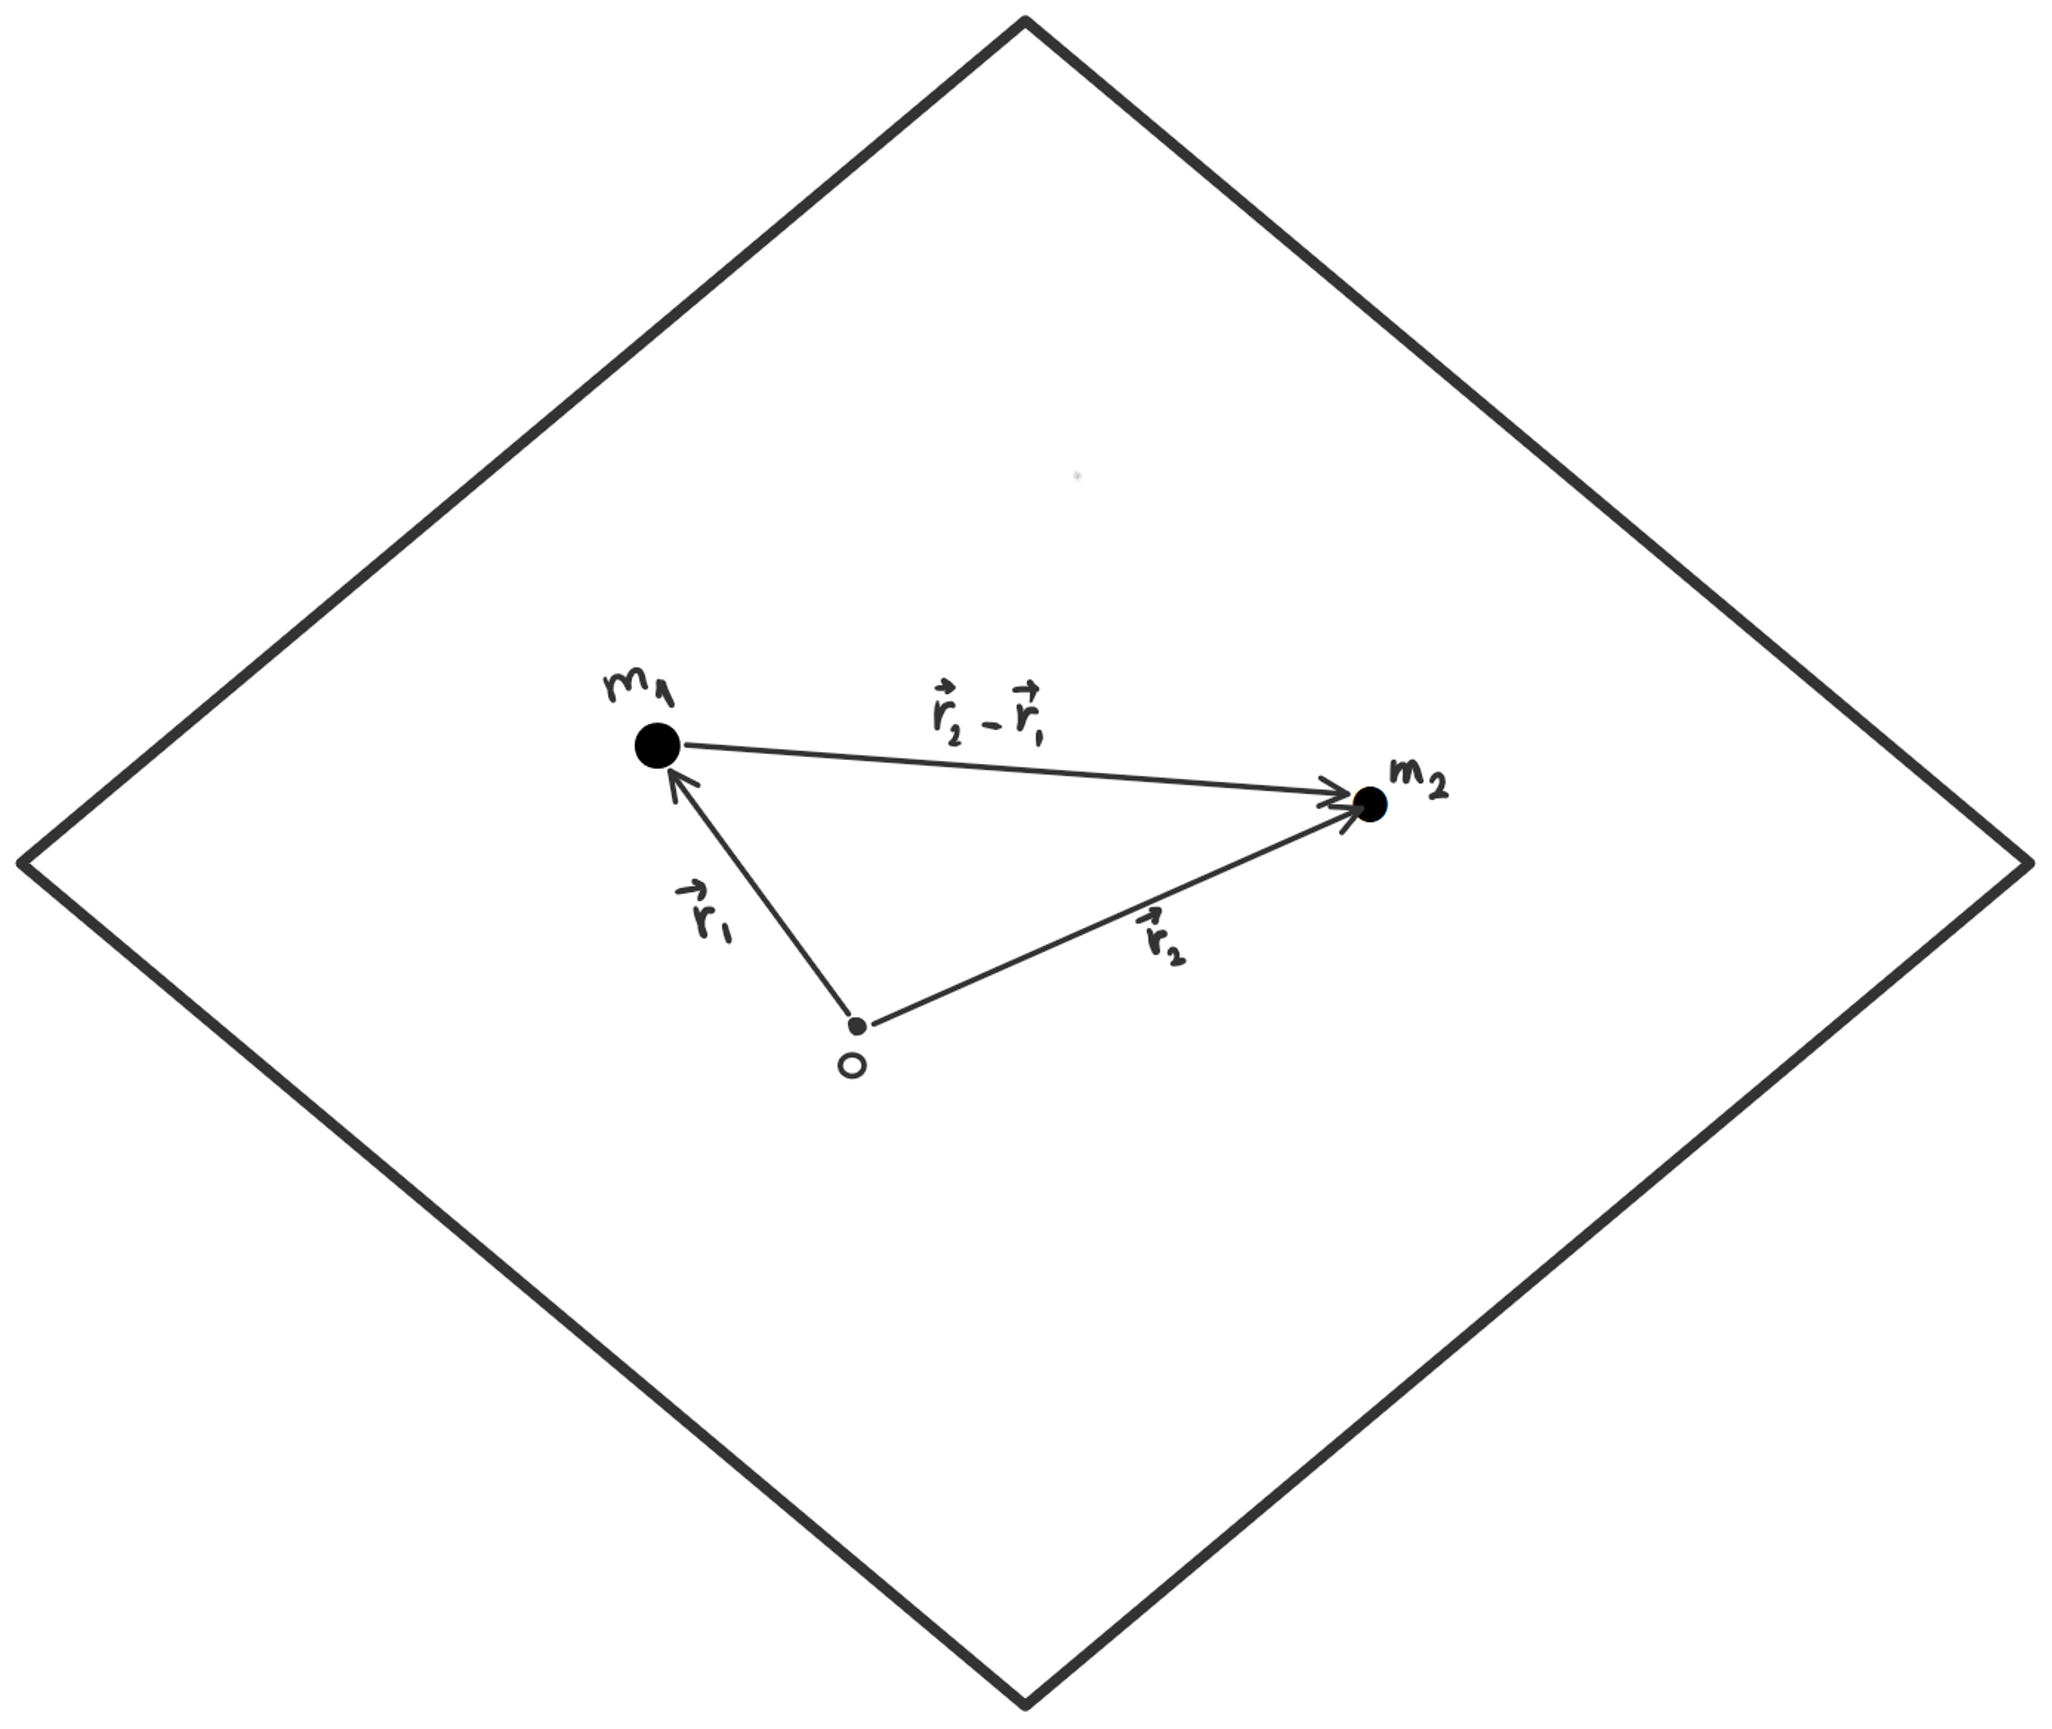
\includegraphics[scale=0.25]{./Images/Newtoni_1} 
 \end{figure}
Using the polar coordinate we have,
\be
\vec{r} = r \hat{r} \longrightarrow \dot{\vec{r}} =  \dot{r} \hat{r} + r \dot{\hat{r}} =  \dot{r} \hat{r} + r^2 \dot{\theta} \hat{\theta}\longrightarrow \ddot{r} =  \hat{r} (\ddot{r} - r \dot{\theta}^2) + \hat{\theta} (2 \dot{r} \dot{\theta} + r \ddot{\theta})
\ee
So,
\be
2 \dot{r} \dot{\theta} + r \ddot{\theta} = 0 \longrightarrow \dfrac{d  (r^2 \dot{\theta})}{dt} = 0 \longrightarrow r^2 \dot{\theta} = L =const
\ee
Moreover,
\be
\vec{r} \times \dot{\vec{r}} = r \hat{r} \times (\dot{r} \hat{r} + r \dot{\theta} \hat{\theta}) = r^2  \dot{\theta} \, \hat{r} \times \hat{\theta} = r^2  \dot{\theta} = const
\ee
So we can solve the problem in 2 dimensions since the vector perpendicular to the surface including two masses is constant. The equation of motion for the relative vector reads,
\be
\ddot{r} - r \dot{\theta}^2 = - \frac{G M } {r^2} \longrightarrow \ddot{r} - \frac{L^2}{r^3}  = - \frac{G M } {r^2}
\ee
where $M= m_1+ m_2$. Changing time out for $\theta(t)$ and transforming $r(\theta(t))$ to $u(\theta(t))=1/r(\theta(t))$ we get,
\be
u'' + u- \frac{G M }{L^2} =0
\ee
To obtain angle as a function of time we have another equation from conservation of angular momentum,
\be
\frac{d \theta}{d t} = L u^2 \longrightarrow  t-t_0= \int_{\theta_0}^{\theta}  \frac{L}{u^2(\theta)} \, d\theta
\ee
For the purpose of our work we use the angle as a free parameter and also we do not solve the equation to obtain the time, since the angle is enough to obtain the perihelion and accepting it as a free variable helps us to simplify our problem.
\subsection{Strong/weak regime way I}
To go in different regime we define a parameter $\alpha$ which scales the physical quantities as following,
\begin{align}
&M \rightarrow \alpha M \\
 &v_{per} \rightarrow \sqrt{\alpha} v_{per}  \\
 &T \rightarrow \dfrac{T}{\sqrt{\alpha}}
\end{align}
which are consistent with centripetal force formulas
\be
v=\frac{GM}{R}, \; \; \; \; \; T= \frac{L}{v}
\ee
$T$ is the object's period, $v_{per} $ is the perihelion speed of the object and $M$ is the central object's mass. By $\alpha$ we can go to the strong/weak limit  while keeping one period orbit in time $\dfrac{T}{\sqrt{\alpha}}$ .
\\
The initial conditions for the problem are,
\begin{align}
&x_0=R \\
&y_0=0 \\
&v_x= \,v_{per}\\
&v_y=0
\end{align}
To compare the results with Mercury observations we use Mercury's facts %\ref{facts}
\begin{align}
&M_{mercury}=3.285 \times 10^{24}  \text{  kg}\\
&T=87.96 \text{  days}\\
&v_{per}=58.98 \text{  $k m/s$}\\
&R=46 \times 10^9   \text{  $ m$}\\\
&M_{sun}=1.99 \times 10^{30}  \text{  $ kg$}\\\
\end{align}
\subsection{Strong/weak regime way II}

The second way we can interpolate is by changing the distances and keeping masses constant as following,
\begin{align}
&M \rightarrow  M \\
 &R \rightarrow  \beta {R} \\
 &T \rightarrow \beta^{3/2} {T} \\
 &v_{per} \rightarrow  \frac {  v_{per}  } {\sqrt{\beta}}
\end{align}
R is the perihelion radius.
The initial conditions for the problem are,
\begin{align}
&x_0=\beta R \\
&y_0=0 \\
&v_x=  \, \frac{v_{per}}{\sqrt{\beta}}\\
&v_y=0
\end{align}
We choose second way of rescaling since the distances are very important for us, because of another length scale in the problem which is lattice grids length.

\subsection{code:}
We use Radau5 code to solve the differential equation and getting the perihelion advance. In the code we solve the below equations,
\be
u'=v_{u}, \; \; v'_{u}=-u + GM/L^2
\ee
 the code for mercury like object is as following,
  \begin{lstlisting}[language=FORTRAN,
  basicstyle=\tiny]
!#############################
  !FILE OPEN
  !#############################
  !!  open (unit = 12, file = "datajp.dat")

!#############################
  !End points
  !#############################
  ! --- endpoint of integration
  ! ------ obligatoire au debut -------
  xbeg=0d0
  xend=200d0
  !####################################################
  !##########Initial values FOR SCHWARZCHILD,
  ! ##########we start from prehelion values
  !####################################################
  !#### y(1) = u(ini) =1/R =0.021739130434782608695652173913043478260869565217391
  !#### u'(ini) = 0
  y(1)=1.d0/(46.d0)
  y(2)=0
  ! --- required tolerance
  !       rtol=1.0q-20
  !       atol=1.0q-7*rtol
  rtol=1.0q-22
  atol=1.0q-22
  itol=0
  ! --- initial step size
  h=1.0d-4
  
  real*16 rr,xx,yy
    real*16 twopi
    twopi=2.* 3.1415926535897932384626433832795028841971693993751q0
    advance=0.00001115996
    if(nr==1)then
       xold=x
       lastx=0
       oldderivative=1
       return
    endif
    dt=0.1d00

  dt=0.001d00
  !  print *,'diff',x-lastx,x,lastx
  if(x<=lastx) then
     print *, '???',x,lastx
     stop
     return
  endif
  nrpts=(x-lastx)/dt
  !print *,nrpts,lastx,x

  !
  !############PRINTING#####################
  !#########################################
  !  print *,'x=',x,'lastx=',lastx,'pts=',nrpts
  if(nrpts<=0)return
  do i=1,lrc
     rccopy(i)=rc(i)
  enddo
  do i=1,lic
     iccopy(i)=ic(i)
  enddo
  do i=1,nrpts
     t=lastx+i*dt
     !print *,oldderivative,derivative(x),x
     if(derivative(t-dt) >0.and.derivative(t)<0)then
        lrccopy=lrc
        zerotime=zeroin(t-dt,t+dt,derivative,0Q00)

        !######################################
        !####This will print the minimum and the angle
        !######################################
        !print *,mod(zerotime,twopi)
                
        oldderivative=derivative(t+dt)
     endif
     !  lastx=x
     rr=1/contex(1,t,rc,lrc,ic,lic)
!     print *,rr
!     stop
     xx=rr*cos(t)
     yy=rr*sin(t)

     !######################################
     !###We can print the orbit easily by following command
     !######################################
     print *,xx,yy

  enddo
  lastx=t
  oldderivative=derivative(t)

  !   print *,'lastx=',lastx
  return
!  close(12)
end subroutine solout
!
!
!cccc  the vector field for
!c van der pol

!####################################################
!###########Differential Equation Adding
!####################################################
subroutine vf(n,x,y,f,rpar,ipar)
! --- right-hand side of equ
include 'sample.h'
integer*4 n,ipar
real*16 x,rpar
real*16 y(n),f(n)
!     y(1) = u(r), y(2)=u(phi)
!     phi is the indepndent variable in radiant
!     (u,uv) in Shcw case
!(u'=v , v' = -u + GM/L^2 + 3/2 R_sch u^2 )

!####################VARIABLES###############
!###### alpha = rescale the problem, mass of sun and maximum velocity.
!#######################################
real*16 G, c, Mearth, Lm, MSun, vmax, Radius, Lsquared, Rsch, GML2, alpha

!#####################################################
alpha=1d0 ! was 1d4
Mearth = 5.972*1.d24 !(*kg*)
MSun = 1.99 * 1.d30 * alpha/Mearth  !(*kg*) (*Normalized to earth's mass*)
Radius=46.0 !(*Giga meter*)
G = 6.67*1.d-26 * Mearth
c = 2.998 * 1.d5
vmax = 58.98* SQRT(alpha)   !(*(Giga meter)/(Mega second)*)
Lm = Radius * vmax;
GML2=G * MSun/(Lm*Lm)
Rsch=2 * G * MSun/(c*c)

!#####################################################

f(1)=y(2)
f(2)= -y(1) + GML2 + 1.5 * Rsch * y(1) * y(1)
!  print *,y(1),y(2),f(1),f(2)
return
end subroutine vf


subroutine dvf(n,x,y,dfy,ldfy,rpar,ipar)
! --- jacobian
include 'sample.h'
integer*4 n,ldfy,ipar
real*16 x,y,dfy,rpar
dimension y(n),dfy(ldfy,n)
return
end subroutine dvf
!####################################################
!####################################################


subroutine mass(n,am,lmas,rpar,ipar)
  integer*4 n,lmas,ipar
  real*16 am(lmas,n),rpar

  integer*4 j
!    print *,lmas,n

!########## For stiff equations we can put the am to zero for the relavant variable
  do j=1,n-1
     am(1,j)=1
  enddo
  am(1,n)=1
    \end{lstlisting}
    After printing the information of orbit we can plot it with the following command by 
     \begin{lstlisting}[language=Bash,
  basicstyle=\tiny]
  ./make   | xmgrace  -
     \end{lstlisting}
     In the xmgrace we can ask for the residual of perihelion in each round and we get the following plot for Newtonian case,
                 \begin{figure}[H]
 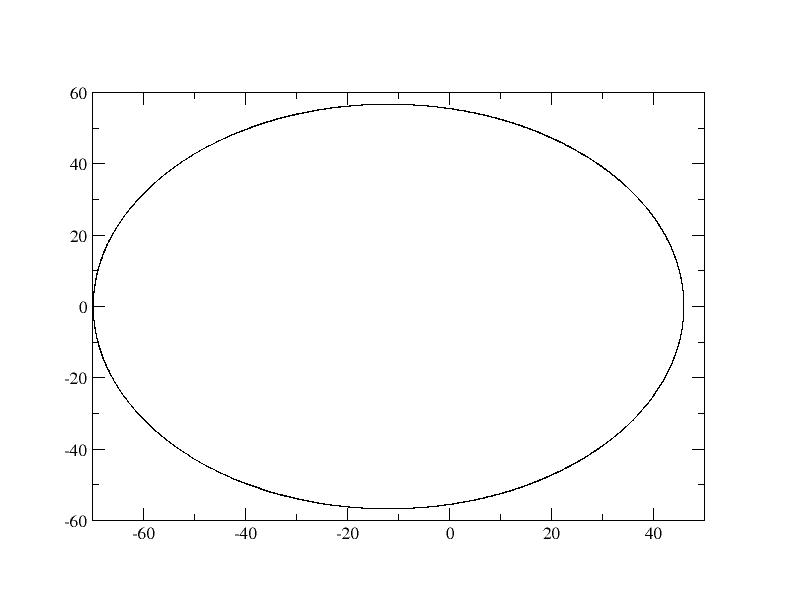
\includegraphics[scale=0.7]{./Images/2.jpg} 
 \end{figure}
            \begin{figure}[H]
 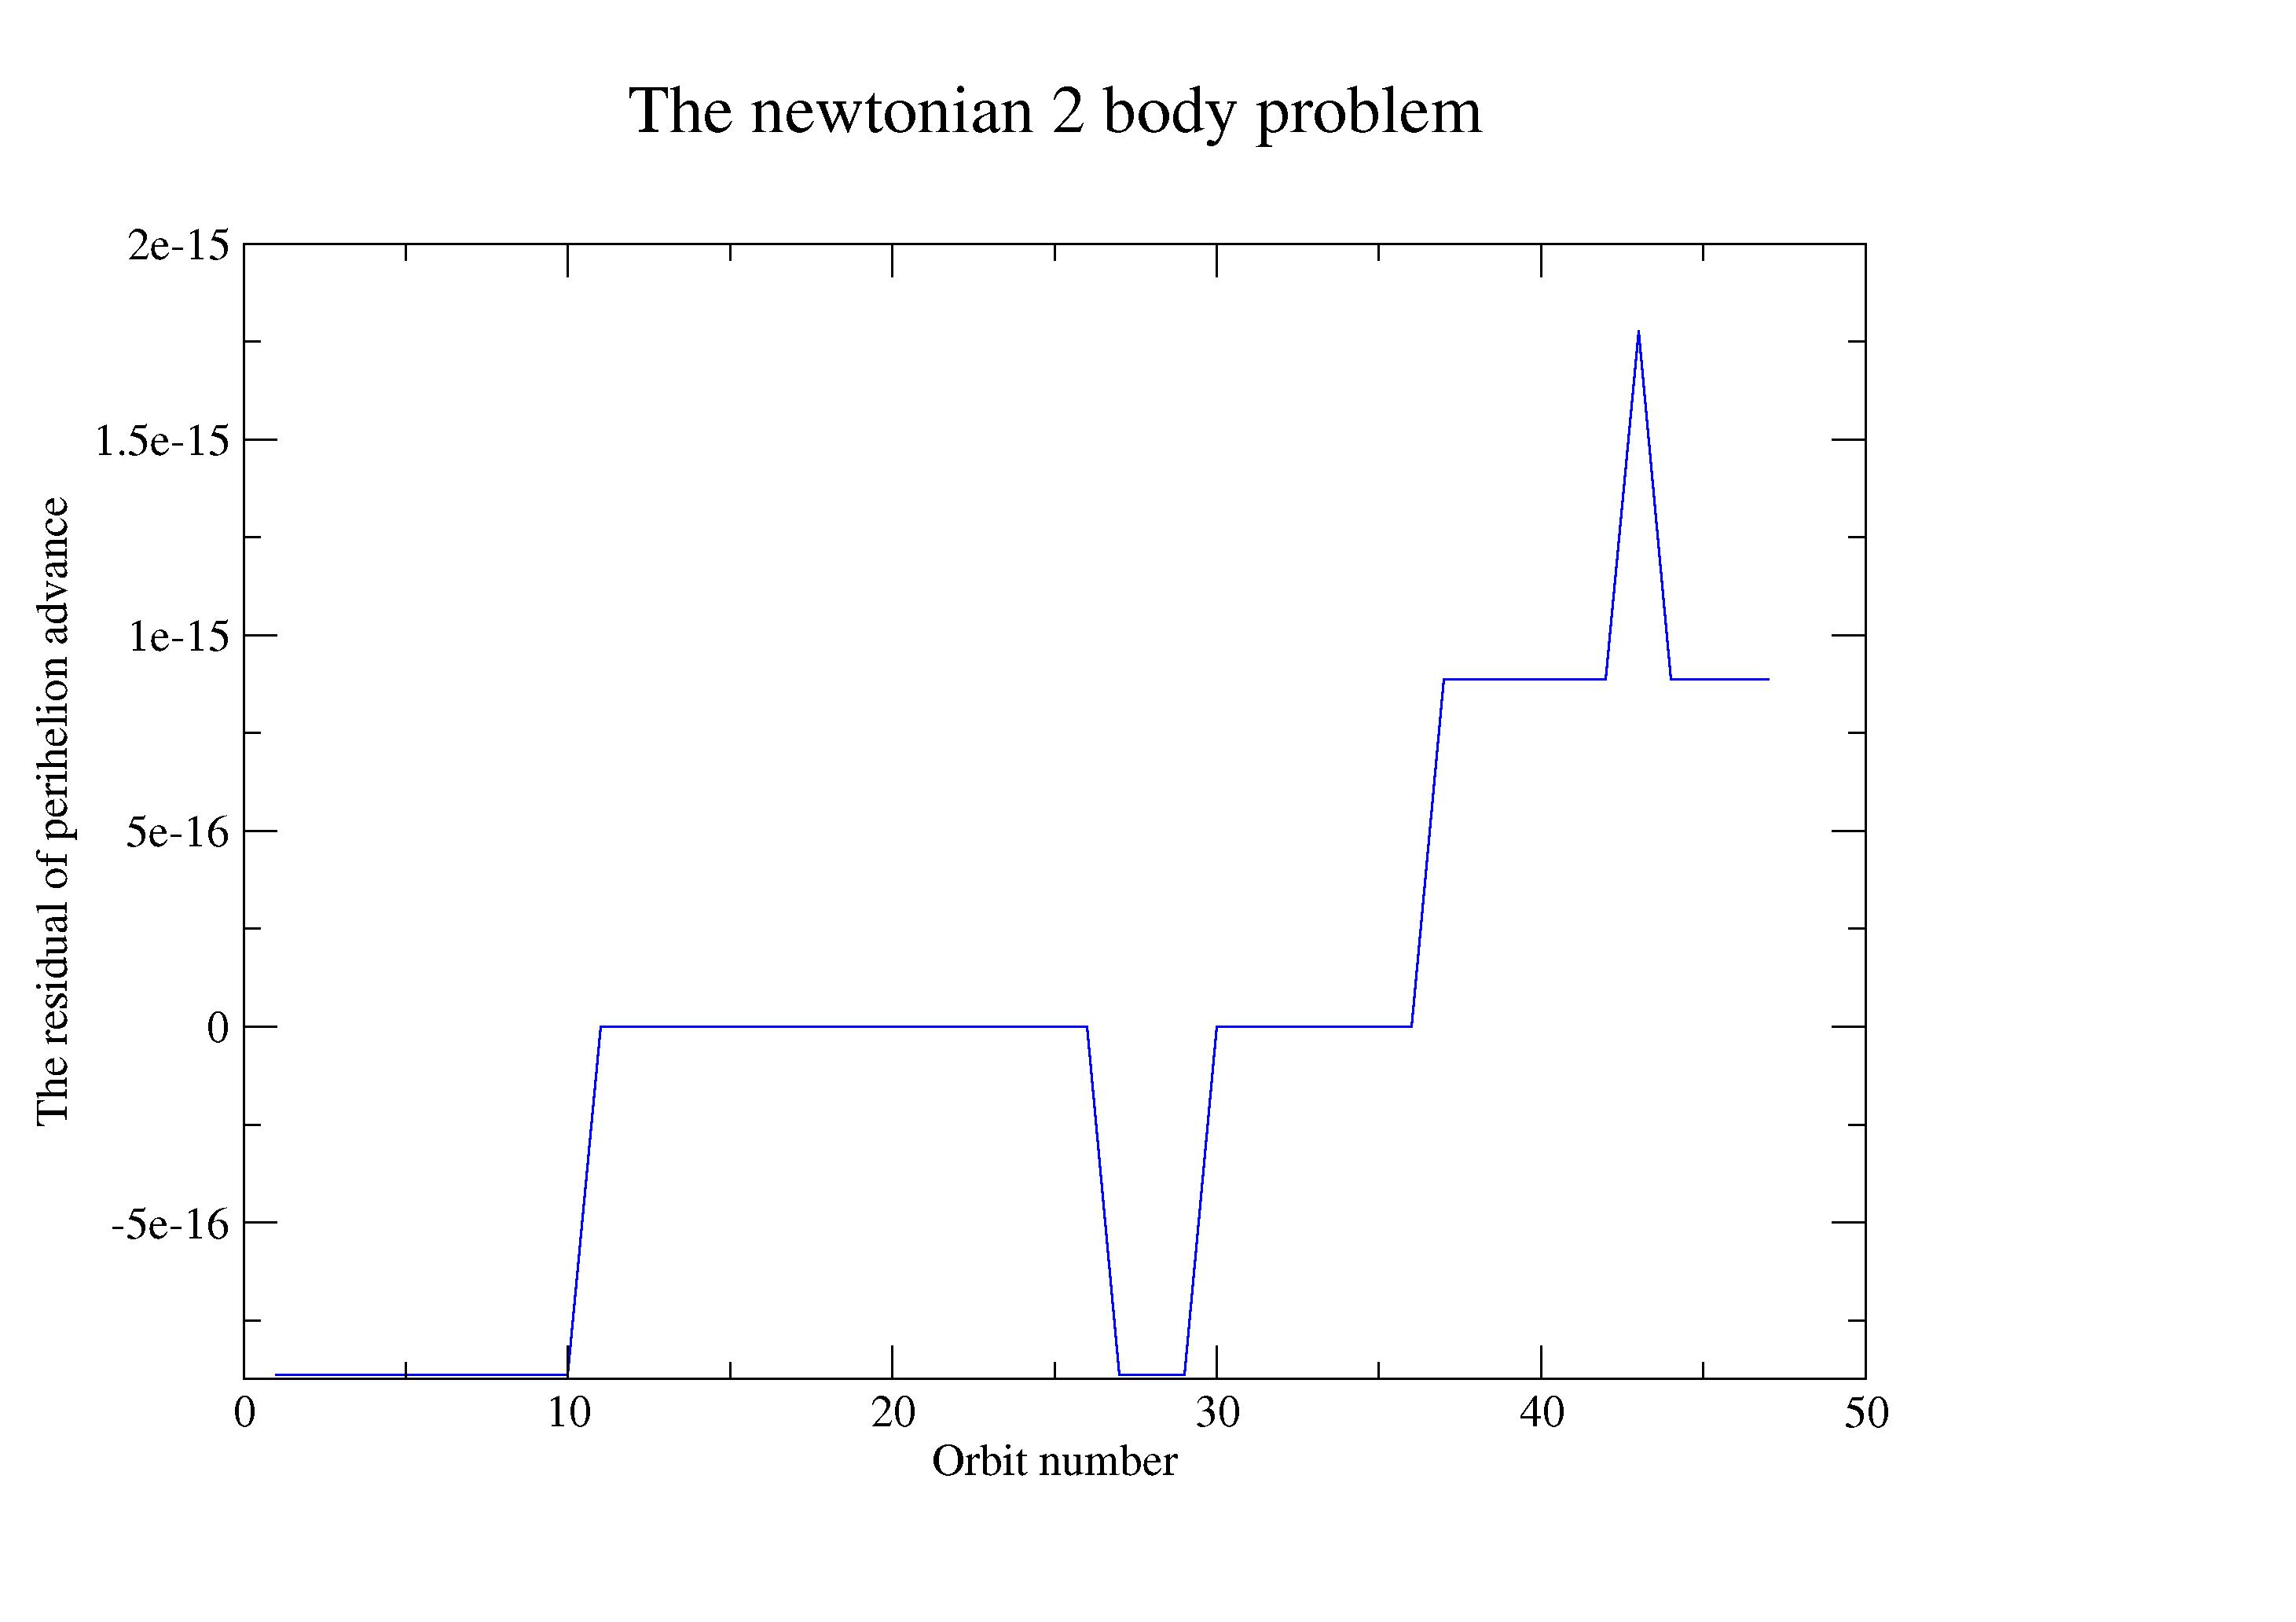
\includegraphics[scale=0.2]{./Images/1} 
 \end{figure}
As it is clear we do not get perihelion advance for Newtonian gravity with the precision of $10^{-15}$, which makes sense.
  \subsection{x-y plane}
  Here we do not use all of the symmetries, we just assume that  the motion is on a plane and we solve the equation for relative distance between two masses,
\be
\dfrac{d^2\vec{r}}{dt^2}=\dfrac{-G  (m+M)}{|r|^3} \vec{r}
\ee
We assume $m \ll M$ so we can simplify as,
\be
(\dot{v_x}, \dot{v_ y})=\frac{-G  M }{(\sqrt{x^2 + y^2})^3}   \; (x,y)
\ee
\be
(v_x, v_ y) = (\dot x, \dot v)
\ee
Now we try to get the same result in this new non-simplified coordinate system. In the code we need to assume $n=4$ which means we have two variables and their derivatives. We also need to have some assumptions for the precision quantities, according to the code below,
  \begin{lstlisting}[language=FORTRAN,
  basicstyle=\tiny]
    ! * * * * * * * * * * * * * * * * * * * * * * * * *
  ! --- driver for seulex16
  ! * * * * * * * * * * * * * * * * * * * * * * * * *

  include 'sample.h'
  ! --- parameters for radau5 (full jacobian)

  ! * * * * * * * * * * * * * * * * * * * * * * * * *
  integer*4 n
  ! Four parameters (x,y,v_x,v_y)
  parameter(n=4)
  integer*4 nd
  integer*4 lwork,liwork,nrdens
  parameter (nd=n,nrdens=n)
  !  parameter (lwork=4*nd*nd+12*nd+20,liwork=3*nd+20)
  parameter (lwork=1000,liwork=1000)
  ! --- declarations
  real*16 y,work
  dimension y(nd)
  dimension work(lwork)
  integer*4 iwork(liwork)
  !     vf is vector field
  !     dvf is tangent map to vector field (when you compute it analytically
  external vf,dvf,solout,mass
  real*16 atol,h,rtol
  integer*4 i,ijac,imas,iout,itol,mljac,idid,mlmas,mumas,mujac,j
  ! could use parameters in function
  real*16 rpar
  integer*4 ipar
  integer*4 ifcn

  !## x is an independent variable
  real*16 x,xbeg,xend
  !     character*40  arg
  !     call getarg(1,arg)
  !     read(arg,'(f7.4)')q2
  !     call getarg(2,arg)
  !     read(arg,'(f7.4)')p2
  !     call getarg(3,arg)
  !     read(arg,'(f7.4)')p3
  ! --- dimension of the system
  !     n
  ! --- compute the jacobian analytically
  ijac=0
  ! --- jacobian is a full matrix
  mljac=n
  ! --- differential equation is in explicit form
  imas=1
  mlmas=0
  mumas=0
  ! --- output routine is used during integration
  iout=1
  ! --- DIMENSION OF THE SYSTEM
  !        N=4
  ! --- PROBLEM IS AUTONOMOUS
  IFCN=1
  ! --- COMPUTE THE JACOBIAN ANALYTICALLY
  IJAC=0
  ! --- JACOBIAN IS A FULL MATRIX
  MLJAC=N
  ! --- DIFFERENTIAL EQUATION IS IN EXPLICIT FORM
  IMAS=0
  ! --- OUTPUT ROUTINE IS USED DURING INTEGRATION
  IOUT=2
  ! --- INITIAL VALUES
  X=0.0Q0

  rpar=0
  ipar=0

  ! * * * * * * * * * * * * * * * * * * * * * * * * *
  !End points
  ! * * * * * * * * * * * * * * * * * * * * * * * * *
  ! --- endpoint of integration
  ! ------ obligatoire au debut -------
  xbeg=0d0
  xend=100q0
  ! --- initial values
  x=xbeg

  do i=1,n
     y(i)=0
  enddo

  ! * * * * * * * * * * * * * * * * * * * * * * * * *
  !FILE OPEN
  ! * * * * * * * * * * * * * * * * * * * * * * * * *
  !!  open (unit = 12, file = "schw_txy.dat")

  ! * * * * * * * * * * * * * * * * * * * * * * * * *
  !Initial values FOR SCHWARZCHILD,
  ! we start from perihelion values
  ! * * * * * * * * * * * * * * * * * * * * * * * * *
  !#### y(1) = x
  !#### y(2) = y
  !#### y(3) = x' =v_x =
  !#### y(4) = y' =v_y =
  !#### we start from y(1)=x= r_mercury and let other variables to be 0
  !#### alpha rescales the problem, masses and ...
  !real*16 alpha , vmax

  ! * * * * * * * * * * * * * * * * * * * * * * * * *
  !alpha=1d0
  y(1)=46.q0 !(Giga meter)
  y(2)=0.q0
  y(3)=0.q0 !(x'=0)
  y(4)= 58.98q0  !(y'= vmax = 58.98 for mercury;//(*(Giga meter)/(Mega !second)*)(*vmax=vmax(1/10^9)(*(Gm/m)*)(10^5/1)*)(*(s/d)*)(*Gm/d*))

  ! --- required tolerance
  !       rtol=1.0q-20
  !       atol=1.0q-7*rtol
  rtol=1.0q-20
  atol=1.0q-29
  itol=0
  ! --- initial step size
  h=1.0d-4
  ! --- set default values
  do  i=1,20
     iwork(i)=0
     work(i)=0.q0
  enddo
  work(1)=1Q-33
  iwork(6)=nrdens
!  print *,iwork(6)
  iwork(2)=3000000
  DO I=1,NRDENS
     IWORK(20+I)=I
  END DO
  ! * * * * * * * * * * * * * * * * * * * * * * * * *
  !  ! * * ALL FOR THE MAIN LOOP
  ! * * * * * * * * * * * * * * * * * * * * * * * * *

  ! --- call of the subroutine radau5
  call seulex(n,vf,ifcn,x,y,xend,h, &
       rtol,atol,itol, &
       dvf,ijac,mljac,mujac,&
       mass,imas,mlmas,mumas, &
       solout,iout,&
       work,lwork,iwork,liwork,rpar,ipar,idid)
  ! --- print final solution
  !        write (6,99) x,y(1),y(2)
99 format(1x,'x =',f5.2,'    y =',2e18.10)
  ! --- print statistics
  write (6,90) rtol
90 format('       rtol=',d8.2)
  write (6,91) (iwork(j),j=14,20)
91 format(' fcn=',i8,' jac=',i8,' step=',i8,&
       ' accpt=',i8,' rejct=',i6,' dec=',i8,&
       ' sol=',i8)
  stop
end program
!

real*16 function derivative(t)
  implicit none
  real*16 t
  real*16 distance
  integer*4 lrccopy,liccopy
  real*16 rccopy(1000)
  integer*4 iccopy(1000)
  common rccopy,lrccopy,iccopy,liccopy
  integer*4 i
  real*16 dt
  !Time step for time derivative
  dt=1.q-18 ! is this a good value
  derivative=(distance(t+dt)-distance(t))/dt

end function derivative


real*16 function distance(t)
  implicit none
  real*16 t
  real*16 contex
  integer*4 lrccopy,liccopy
  real*16 rccopy(1000)
  integer*4 iccopy(1000)
  common rccopy,lrccopy,iccopy,liccopy
  external contex
  ! JPE no
  ! you want the derivative of sqrt(x^2+y^2)
  ! so that is
  real*16 temp(10)
  integer*4 i
  do i=1,2 ! since you are in R^2
  !contex gives the i component at time t and other variables should be there!
     temp(i)=contex(i,t,rccopy,lrccopy,iccopy,liccopy)
  enddo
  distance=sqrt(temp(1)*temp(1) + temp(2)*temp(2))

end function distance

subroutine solout (nr,xold,x,y,rc,lrc,IC,LIC,n,rpar,ipar,irtrn)
  ! --- prints solution at equidistant output-points
  ! --- by using "contex", the continuous collocation solution
  include 'sample.h'
  integer*4 lic
  integer*4 ic(lic)
  integer*4 nr,lrc,n,ipar,irtrn
  real*16 y(n),rc(8),yint(n),rpar,advance
!!!!!! jpadded
  common rccopy,lrccopy,iccopy,liccopy
  integer*4 lrccopy,iccopy(1000),liccopy
  real*16 oldderivative
  real*16 rccopy(1000)
  external derivative
  real*16 derivative
  save lastx,oldderivative
  real*16 zeroin
  external zeroin
  !! end jpadded
  real*16 dt,t
  integer*4 nrpts,i,j
  real*16 x,xold
  real*16 contex
  real*16 lastx,zerotime

    real*16 rr,angle
    real*16 twopi
    twopi=2.* 3.1415926535897932384626433832795028841971693993751q0
    advance=0.00001115996q0
    if(nr==1)then
       xold=x
       lastx=0
       oldderivative=1
       return
    endif

  dt=0.01d00
  !  print *,'diff',x-lastx,x,lastx
  if(x<=lastx) then
     print *, '???',x,lastx
     stop
     return
  endif
  nrpts=(x-lastx)/dt
  !print *,nrpts,lastx,x

  !############PRINTING#####################
  !#########################################
  !  print *,'x=',x,'lastx=',lastx,'pts=',nrpts
  if(nrpts<=0)return
  do i=1,lrc
     rccopy(i)=rc(i)
  enddo
  do i=1,lic
     iccopy(i)=ic(i)
  enddo
  do i=1,nrpts
     t=lastx+i*dt
     !print *,oldderivative,derivative(x),x
     if(derivative(t-dt) <0.and.derivative(t)>0)then
        lrccopy=lrc
        zerotime=zeroin(t-dt,t+dt,derivative,0Q00)

        !######################################
        !####This will print the minimum and the angle
        !######################################
        !print *,mod(zerotime,twopi)
        rr=SQRT( contex(1,zerotime,rc,lrc,ic,lic)*contex(1,zerotime,rc,lrc,ic,lic)&
             + contex(2,zerotime,rc,lrc,ic,lic)*contex(2,zerotime,rc,lrc,ic,lic))
     angle=ATAN(contex(2,zerotime,rc,lrc,ic,lic)/contex(1,zerotime,rc,lrc,ic,lic))
     print *,mod(angle,twopi)
     endif
     oldderivative=derivative(t+dt)

     ! print *,rr

     !######################################
     !###We can print the orbit easily by following command
     !######################################
!     print *,contex(1,t,rc,lrc,ic,lic),contex(2,t,rc,lrc,ic,lic)

  enddo
  lastx=t
  oldderivative=derivative(t)

  !   print *,'lastx=',lastx
  return
!  close(12)
end subroutine solout
!
!
!cccc  the vector field for


!################
!###Function |r|^3 = sqrt(x^2+y^2)^3
!################
real*16 function abscubed(a,b)
REAL*16  a, b
  abscubed= (sqrt(a * a + b*b))**3
!  abscubed=a+b
end function abscubed
!####################################################
!######Differential Equation Adding
!####################################################
subroutine vf(n,x,y,f,rpar,ipar)
! --- right-hand side of equ
include 'sample.h'
integer*4 n,ipar
external abscubed
real*16 x,rpar,abscubed
real*16 y(n),f(n)
!     y(1) = x, y(2)=y
!     time is the independent
!(x'=v_x , v_x'=  -GMx/SQRT(x^2+y^2)^3, y'=v_y , v_y'=  -GMy/sqrt(x^2+y^2)^3 )

!####################VARIABLES###############
!###### alpha = rescale the problem, mass of sun and maximum velocity.
!#######################################
real*16 G, c, Mearth, Lm, MSun, R_perihelion, Lsquared, Rsch, GML2, alpha, vmax


!#####################################################
alpha=1.0
Mearth = 5.972*1.d24 !(*kg*)
MSun = 1.99 * 1.d30 * alpha/Mearth  !(*kg*) (*Normalized to earth's mass*)
R_perihelion=46.0 !(*Giga meter*)
G = 6.67*1.d-26 * Mearth
c = 2.998 * 1.d5
vmax = 58.98* SQRT(alpha)   !(*(Giga meter)/(Mega second)*)
Lm = R_perihelion * vmax;
GML2=G * MSun/(Lm*Lm)
Rsch=2 * G * MSun/(c*c)
!#####################################################

f(1)= y(3) !(x' = v_x)
f(2)= y(4) !(y' = v_y)
f(3)= - G * MSun * y(1)/abscubed(y(1),y(2))   !(v_x' = -GMx/sqrt(x^2+y^2)^3)
f(4)= - G * MSun * y(2)/abscubed(y(1),y(2))   !(v_y' = -GMy/sqrt(x^2+y^2)^3)

!  print *,y(1),y(2),f(1),f(2)
return
end subroutine vf


subroutine dvf(n,x,y,dfy,ldfy,rpar,ipar)
! --- jacobian
include 'sample.h'
integer*4 n,ldfy,ipar
real*16 x,y,dfy,rpar
dimension y(n),dfy(ldfy,n)
return
end subroutine dvf
!####################################################
!####################################################


subroutine mass(n,am,lmas,rpar,ipar)
  integer*4 n,lmas,ipar
  real*16 am(lmas,n),rpar

  integer*4 j
!    print *,lmas,n

!########## For stiff equations we can put the am to zero for the relavant variable
  do j=1,n-1
     am(1,j)=1
  enddo
  am(1,n)=1
  return
  end subroutine mass
  \end{lstlisting}
  some useful terminal commands, to print the result in a file
    \begin{lstlisting}[language=Bash,
  basicstyle=\tiny]
  ./makeit_schw_xy > junk.1st
  emacs junk.1st
  \end{lstlisting}
For $\alpha=1$ which is the case for sun and mercury we get the following perihelion and orbit,
       \begin{figure}[H]
 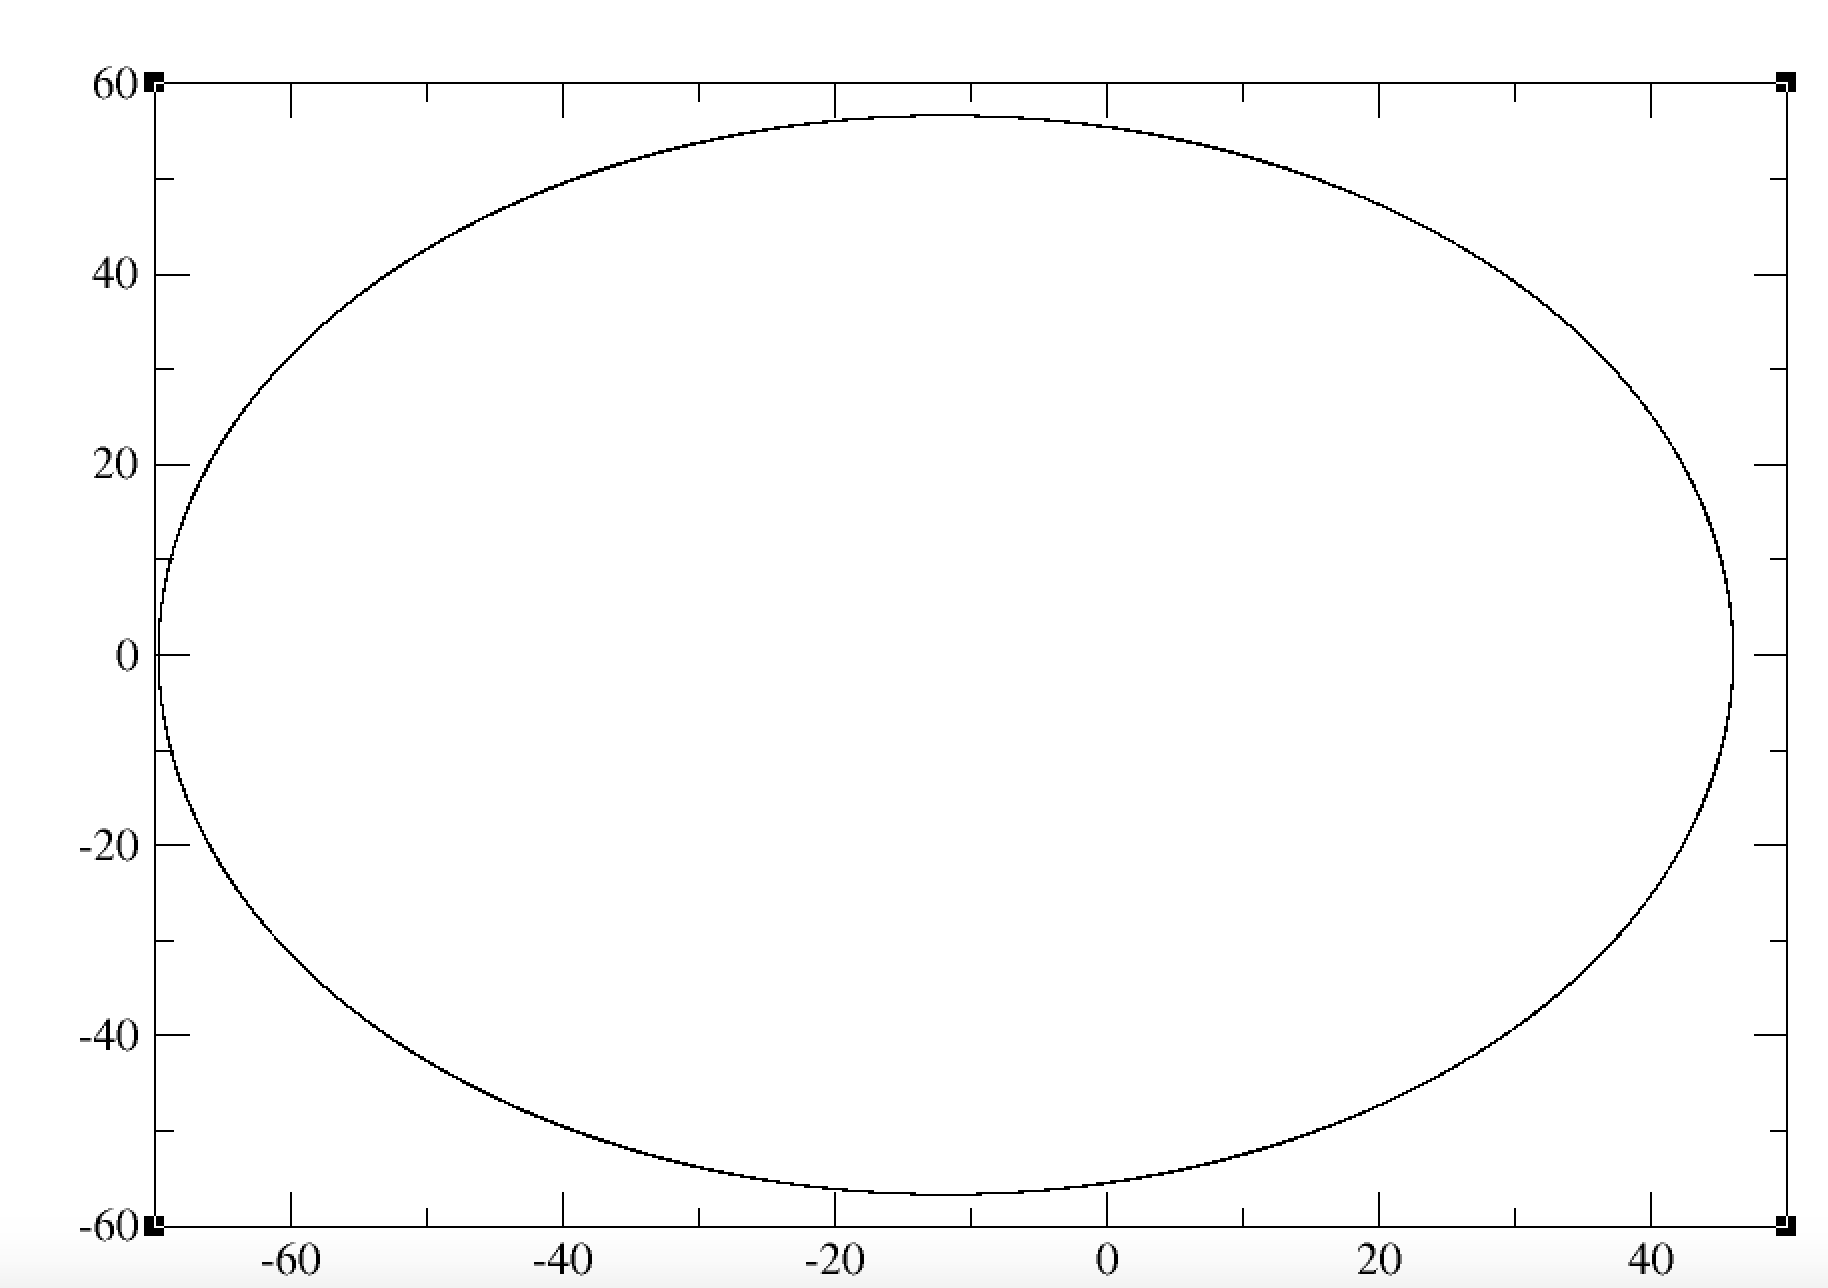
\includegraphics[scale=0.5]{./Images/orbit_xy} 
 \end{figure}
        \begin{figure}[H]
 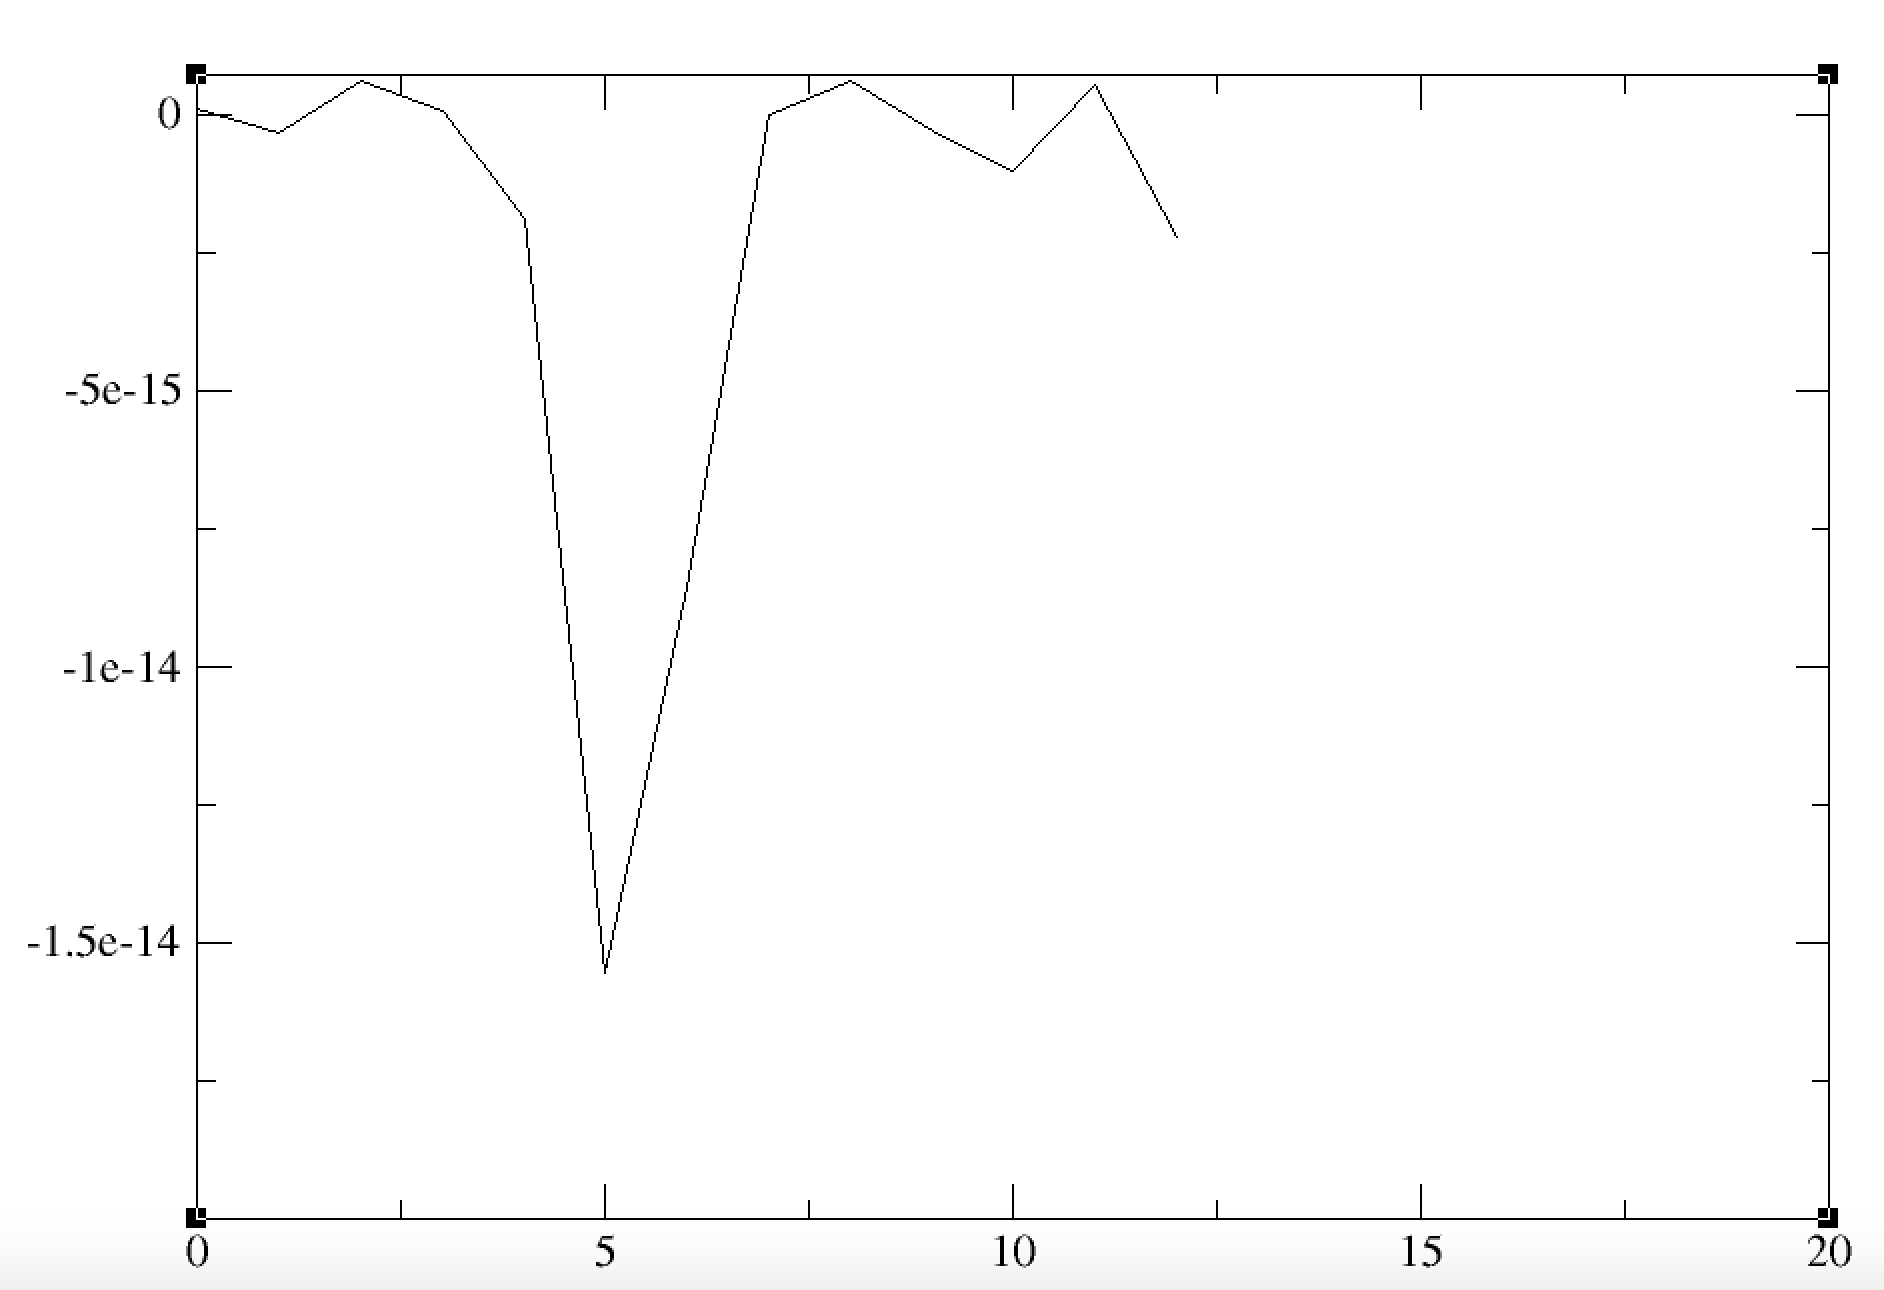
\includegraphics[scale=0.5]{./Images/perihel_xy} 
 \end{figure}
\section{Newtonian gravity on the lattice}
\subsection{2 dimensional case, linear interpolation}
For the first step we solve 2D problem, so basically we have,
       \begin{figure}[H]
 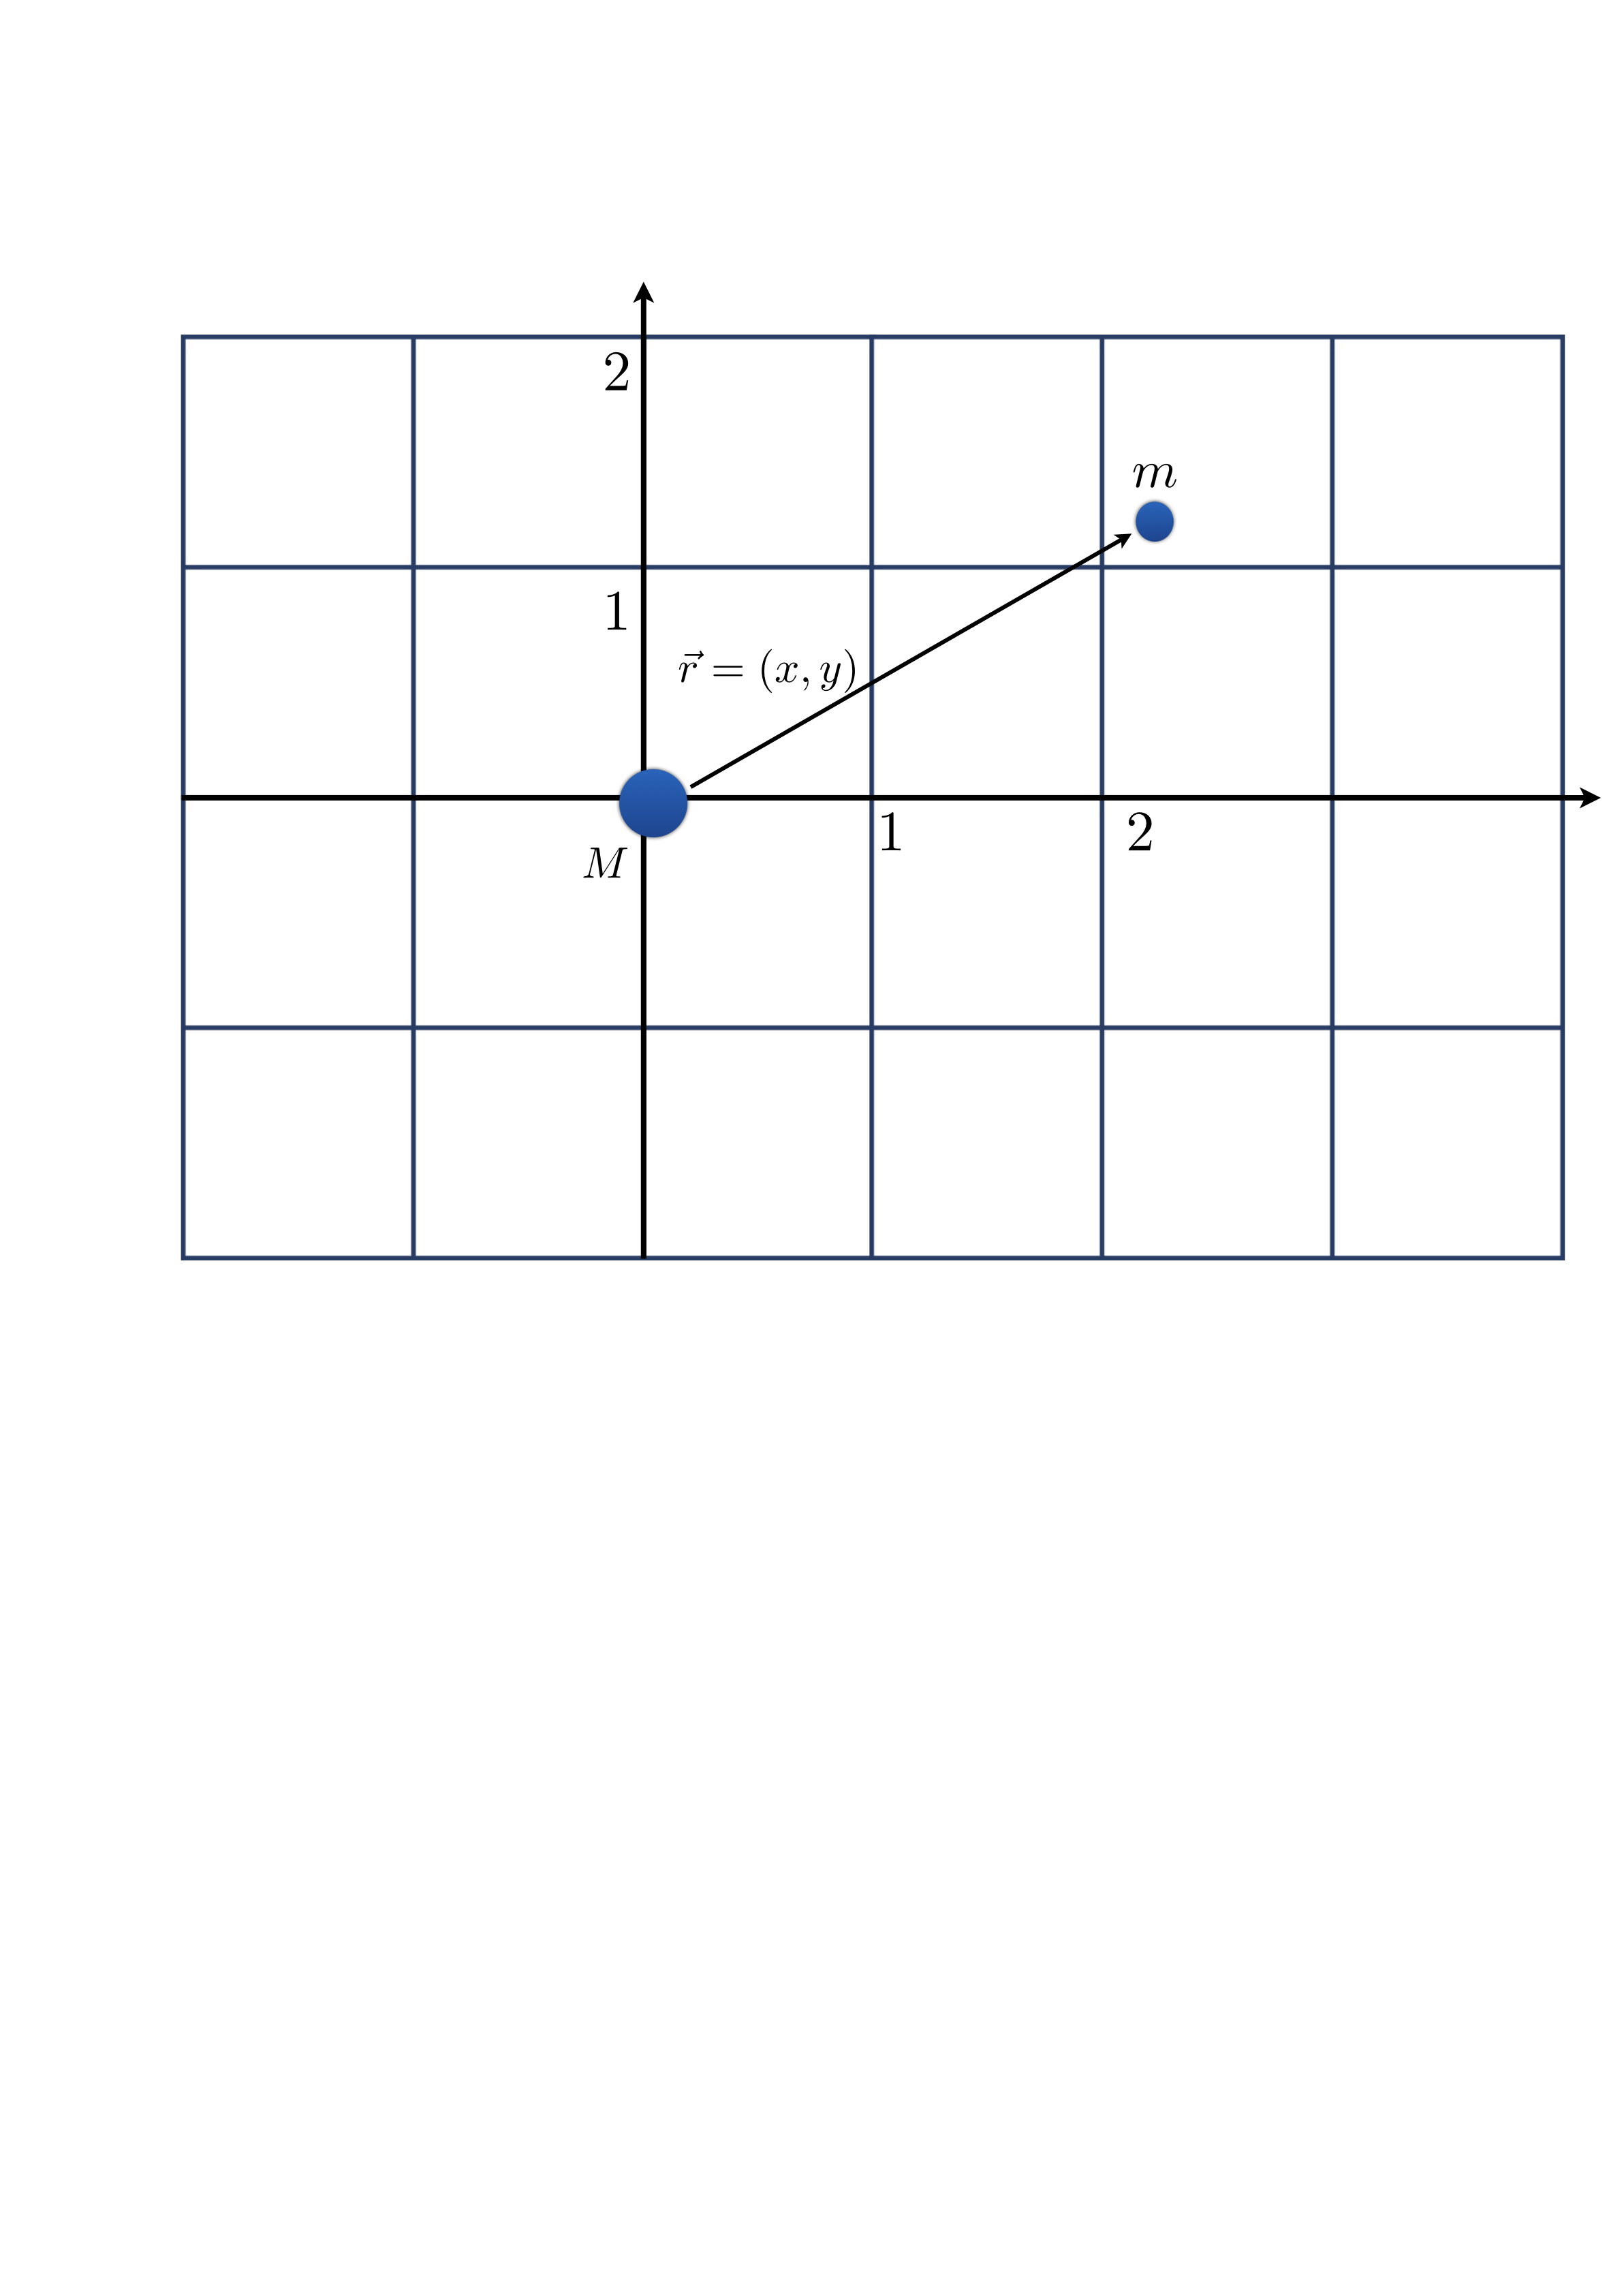
\includegraphics[scale=0.15]{./Images/Image-lattice} 
 \end{figure}
 The potentials of central mass on the cell vertices read,
\begin{align}
 &\Phi_{i,j} = -\frac{G M}{\sqrt{ i^2	 + j^2} }
 \end{align}
 The result of interpolation of potentials at vertices, into the object position is, 
 \begin{align}
& \Phi_{m}(x,y) =\sum_{ (i,j) \, \in \, \text{4 corners}  } \frac{\Phi_{i,j}}{2}  \Big[ \sqrt{1- (x-i)^2} +   \sqrt{1- (y-j)^2}   \Big ]
 \end{align}
 Which we assumed that the interpolation is linear and is ended at the next vertex position, having $ \sqrt{1- (x-i)^2} $ which is 0 at $x=i+1$. At the end the acceleration is,
  \begin{align}
\dot{ \vec v} = \sum_{ (i,j) \, \in \, \text{4 corners}  } \frac{ \Phi_{i,j} }{2}  \;  \Big( \frac{x-i}{\sqrt{1-(x-i)^2} }, \; \frac{y-j}{\sqrt{1-(y-j)^2} }  \Big)
 \end{align}
  \be
 \vec v = \big( \dot x , \dot y\big)
 \ee
There are some notes at this level, first the situation is singular at the lines  $x=i+1, y=j+1$ so we basically we don't expect to get a good result with this interpolation which just cut the forces at the boundaries. But just assume that we just remove singularities by hand in a condition. \\
What happens is if the particle starts from the initial condition (46,$\epsilon$) which is for mercury because of strong force from the boundaries it just oscillates around the boundary.
       \begin{figure}[H]
 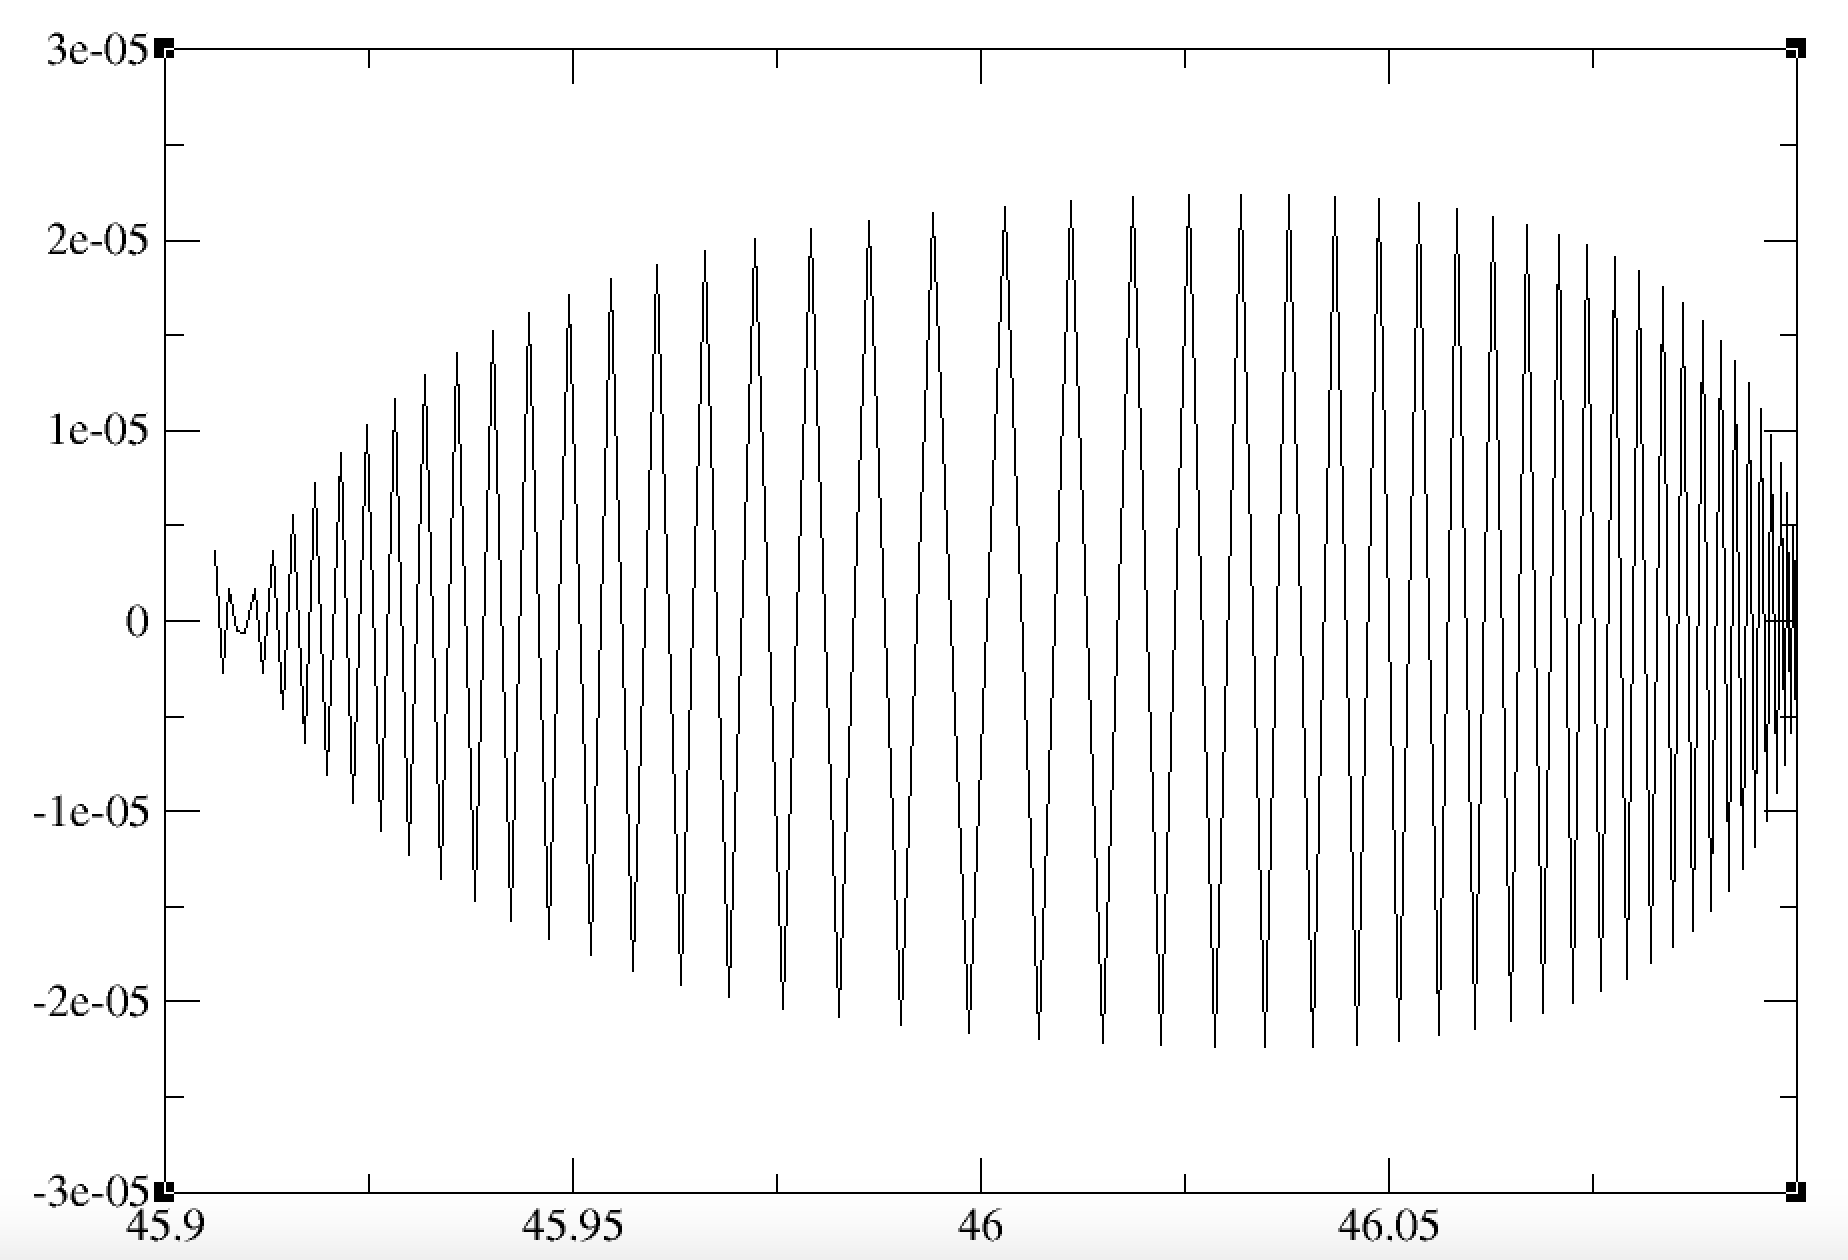
\includegraphics[scale=0.5]{./Images/Lattice_effect_Newtonian_v1} 
 \end{figure}
For any point in the lattice like $(46.4,0.4)$.. we see the same oscilation arround the boundary with the amplitude of distance from boundary,
     \begin{figure}[H]
 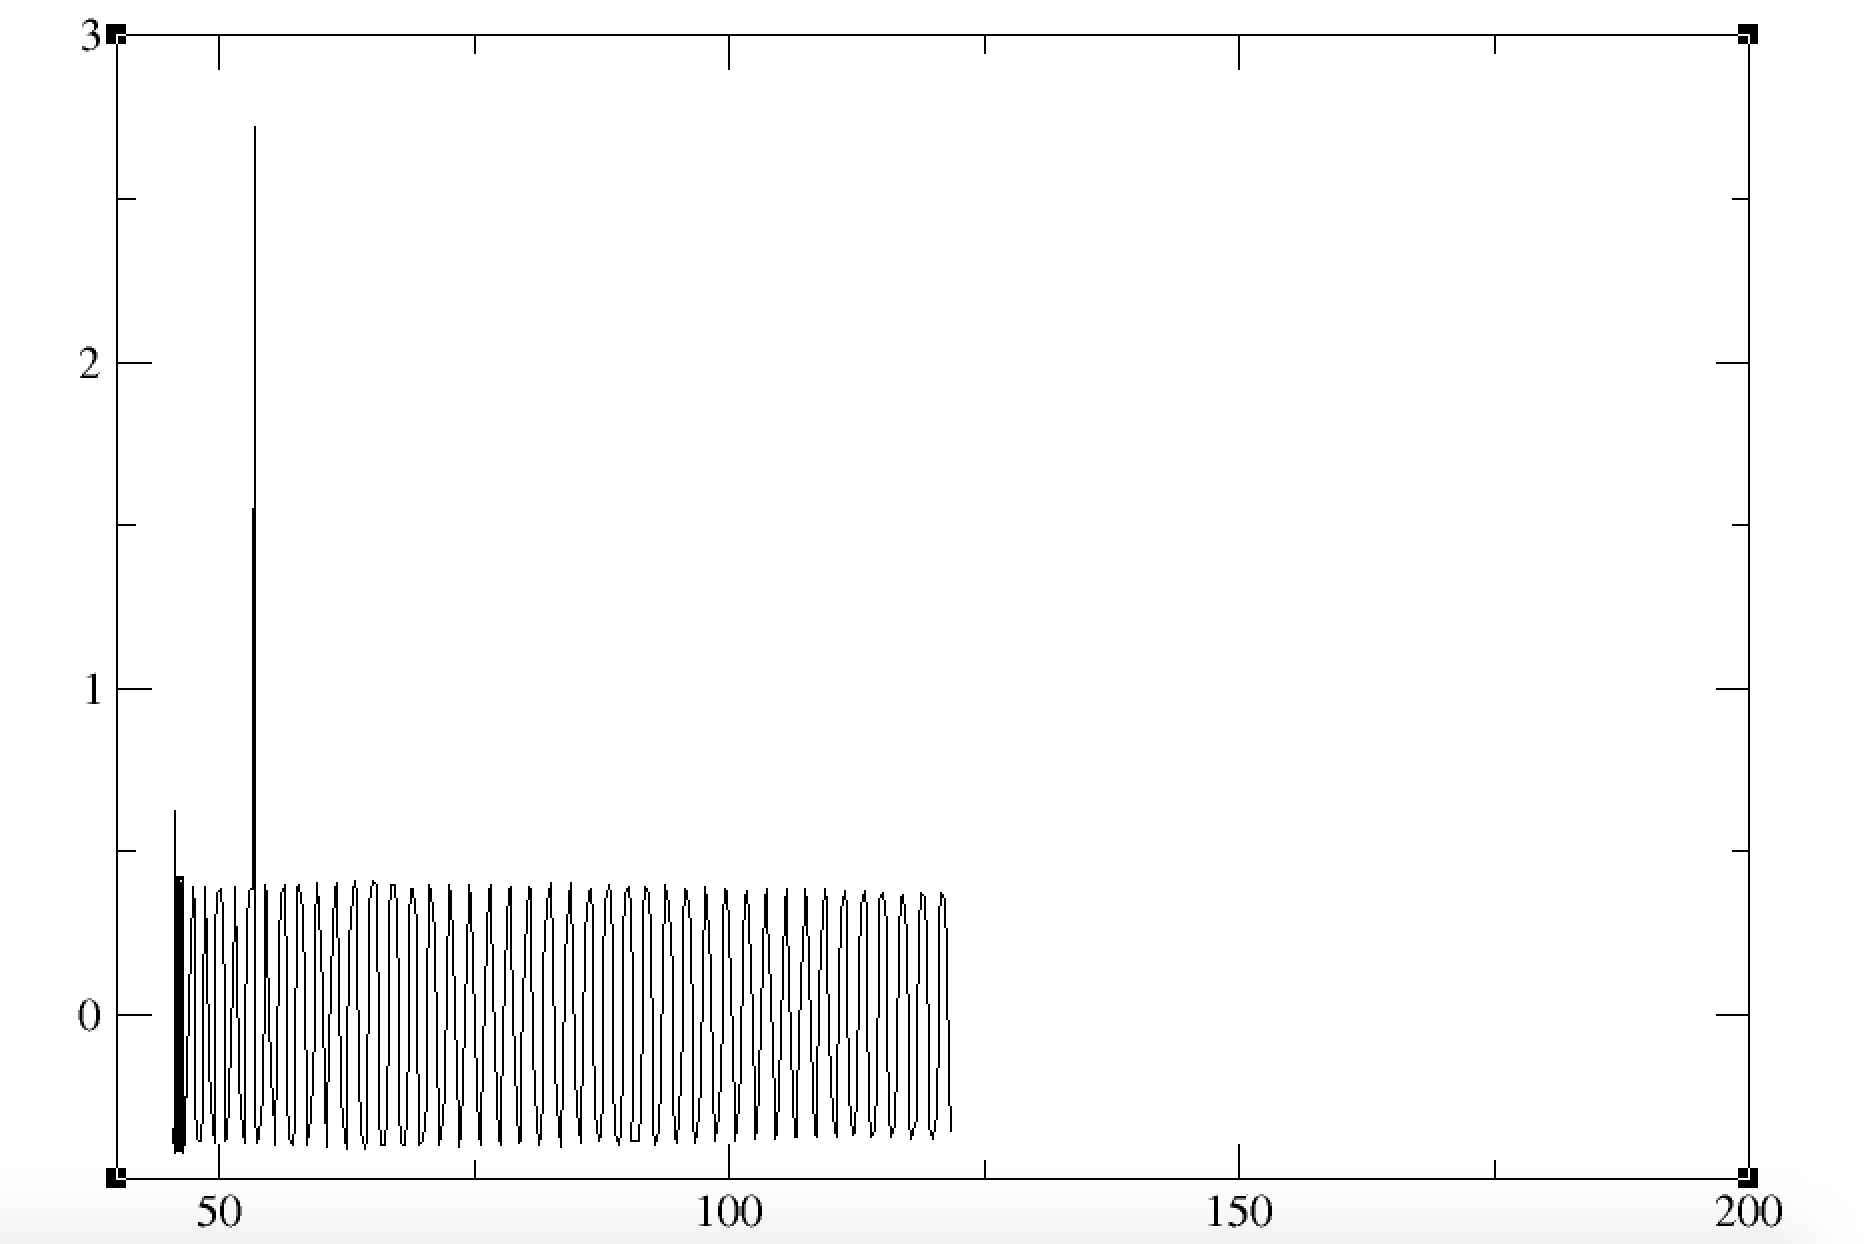
\includegraphics[scale=0.5]{./Images/Lattice_effect_Newtonian_v1_002} 
 \end{figure}
 But for the center of the cell meaning $(46.,0.5)$ we see because of symmetry the particle is not attracted to any cell boundaries and just continue to move with the initial velocity.
     \begin{figure}[H]
 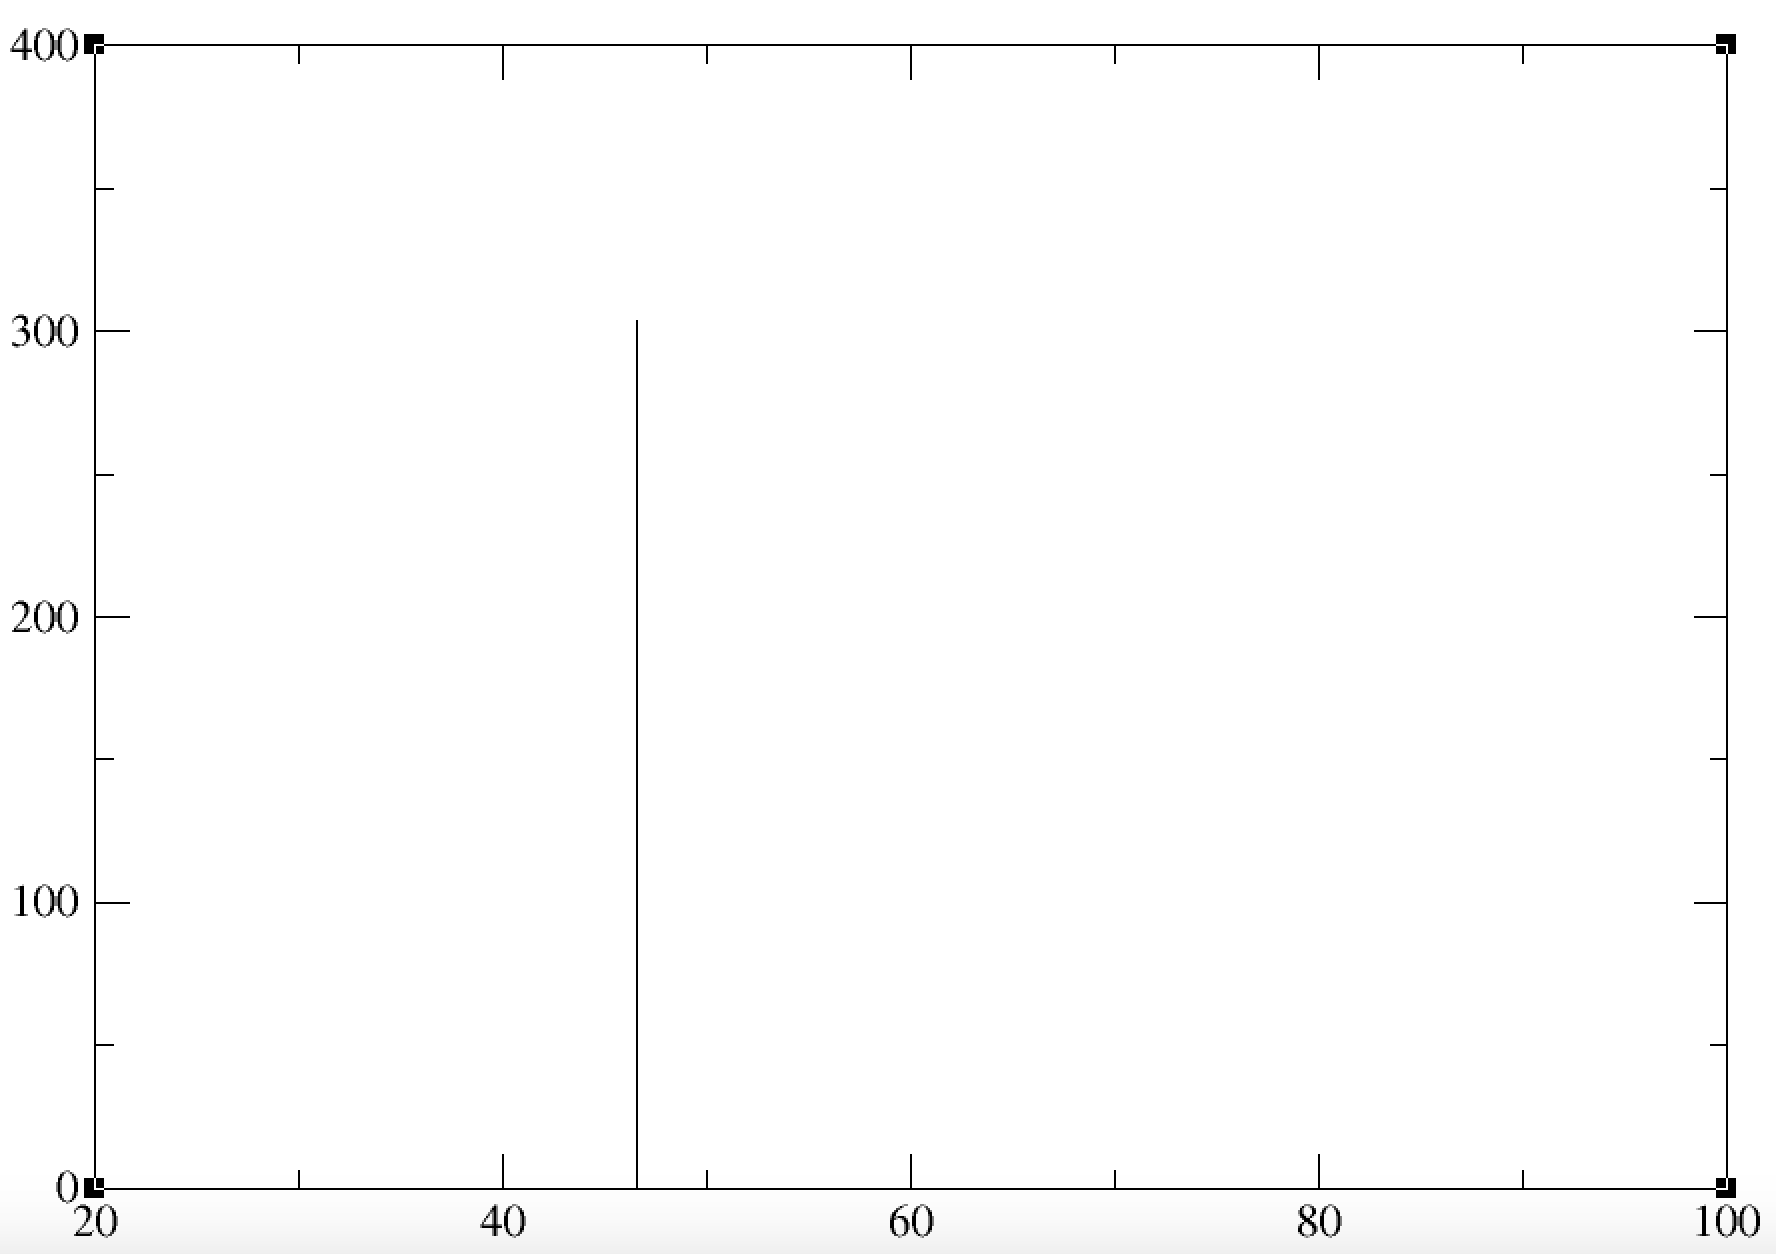
\includegraphics[scale=0.45]{./Images/Lattice_effect_Newtonian_v1_003} 
 \end{figure}

 \subsection{2 dimensional case, computing force}
For the first step we solve 2D problem, so basically we have,
       \begin{figure}[H]
 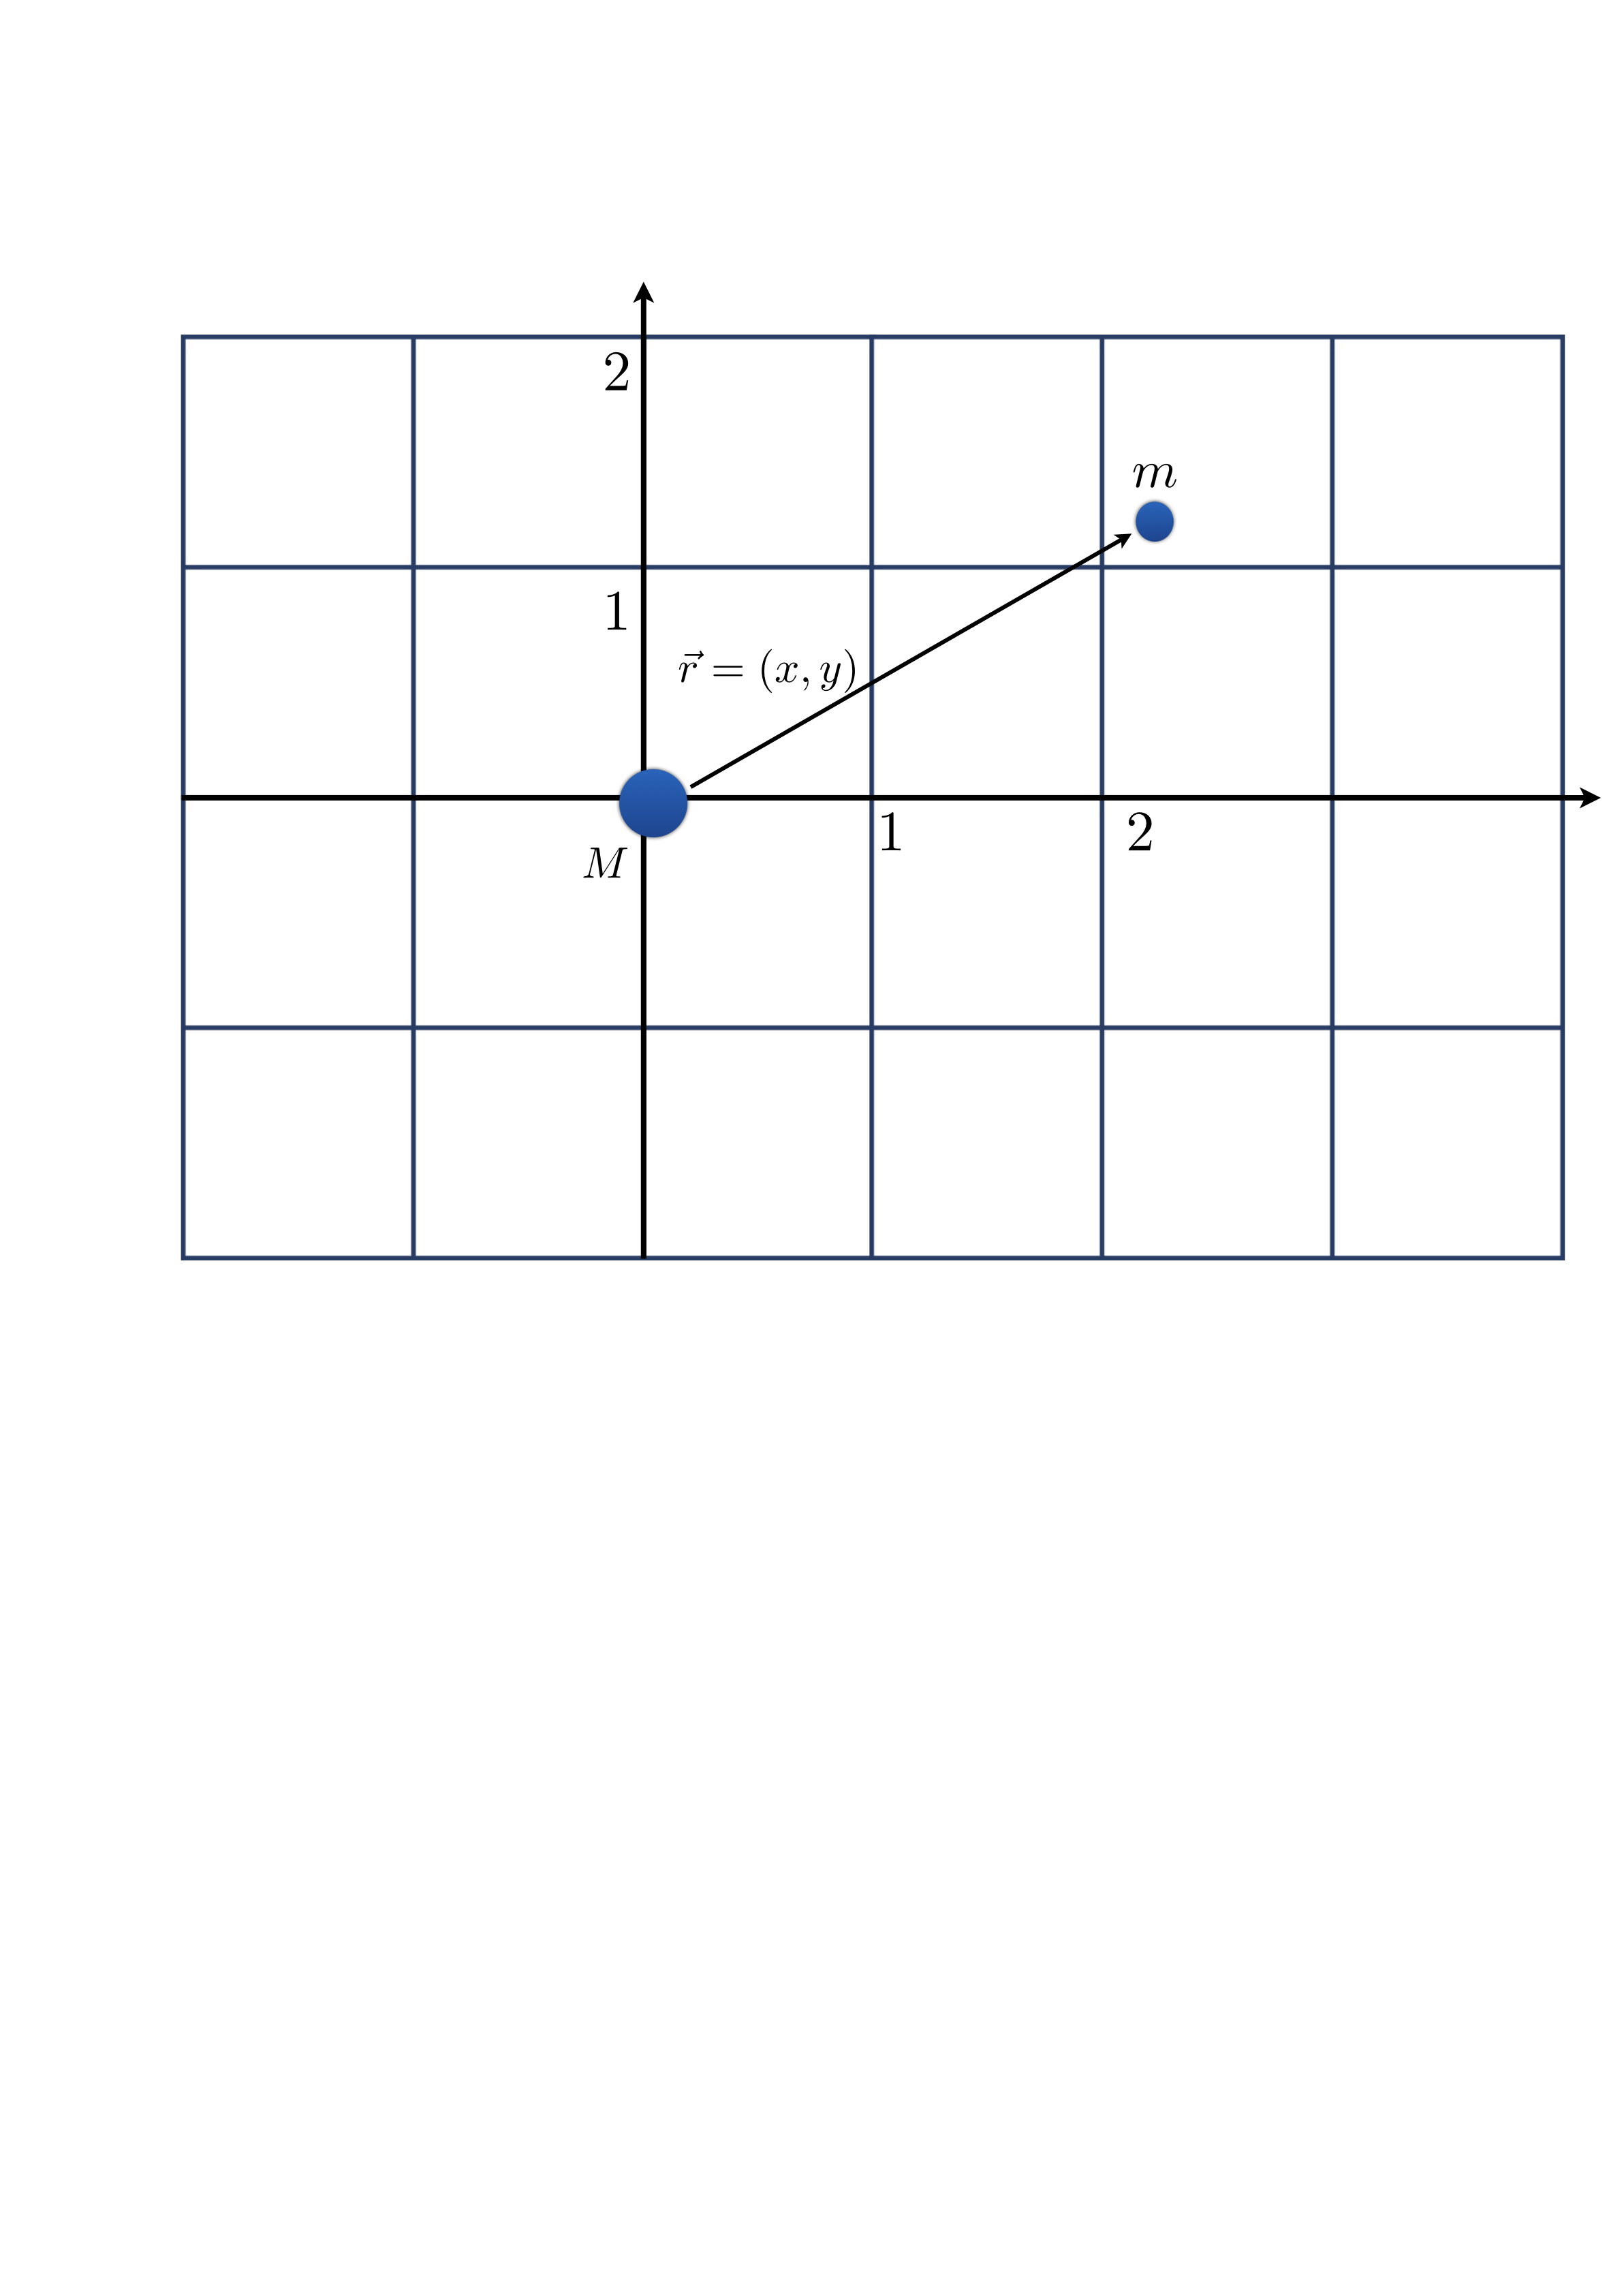
\includegraphics[scale=0.15]{./Images/Image-lattice} 
 \end{figure}
 First we assign masses to the vertices of the cell and the then compute the force from the masses on the particles position,
\begin{align}
 &m_{i,j} = \frac{ M}{\sqrt{ i^2	 + j^2 }}
 \end{align}
 \begin{align}
& \Phi_{m}(x,y) =\sum_{ (i,j) \, \in \, \text{4 corners}  } \frac{-G m_{i,j}}{  \sqrt{(x-i)^2 + (y-j)^2}    } \end{align}
The mass is assigned to the vertices of the cell according to the distance of the vertex ti the central mass,
  \begin{align}
\dot{ \vec v} = \sum_{ (i,j) \, \in \, \text{4 corners}  }   G m_{i,j}\;  \Big( \frac{x-i}{  \Big ( {(x-i)^2 + (y-j)^2}     \Big ) ^{3/2} }, \; \frac{y-j}{  \Big ( {(x-i)^2 + (y-j)^2}     \Big ) ^{3/2}}   \Big)
 \end{align}
  \be
 \vec v = \big( \dot x , \dot y\big)
 \ee
 This procedure also has the same problem as before, which in the boundaries we see some bad behaviors, 
 \subsection{2D calculation-Mistakes}
 Up to now  we were computing the force and potential in the position of particle then we took the gradient, but this method does not converge to the right solution. In the correct method we need to compute the gradient on the cell as well. The gradients are defined in the half of each cell and we have, we start from one way derivatives,
 \be
 \nabla \Phi =\frac{\Phi(\vec x+\vec dx) - \Phi(\vec x) }{dx}
 \ee
 So $\nabla \Phi$ is field in the cell, lives in the half of each side. Again we have the same expressions,
   \begin{figure}[H]
 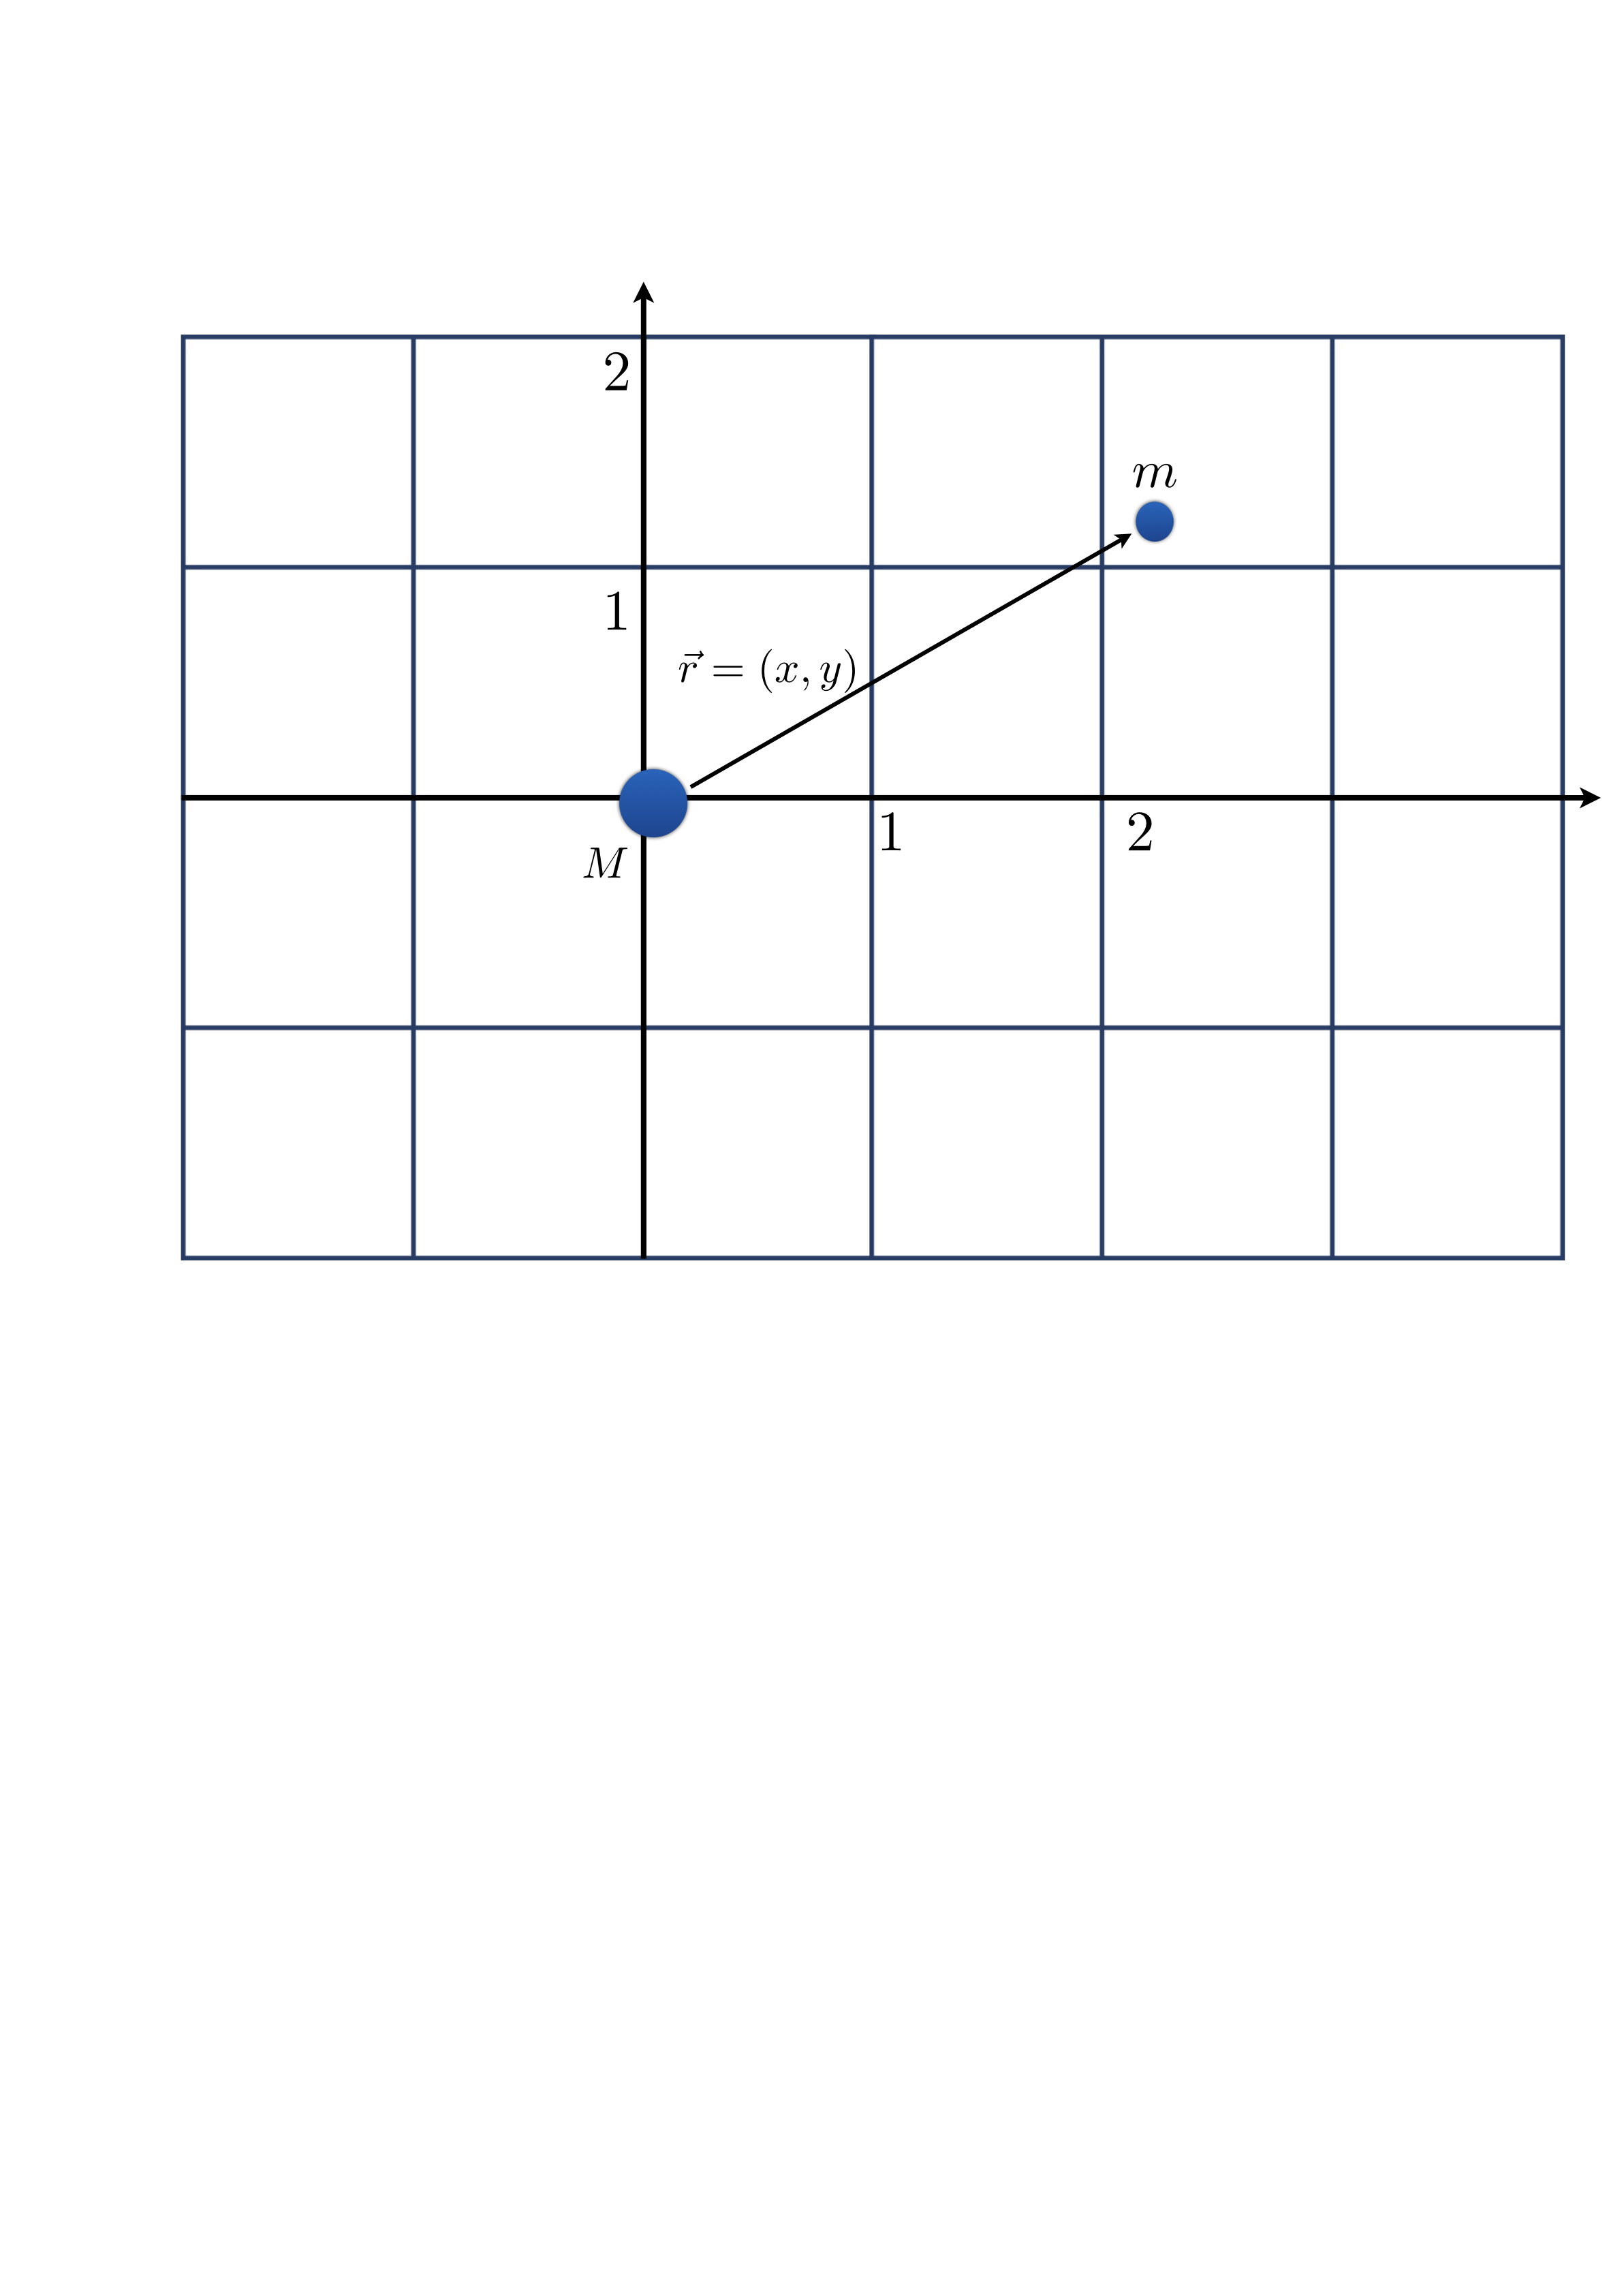
\includegraphics[scale=0.15]{./Images/Image-lattice} 
 \end{figure}
 The potentials of central mass on the cell vertices read,
\begin{align}
 &\Phi_{i,j} = -\frac{G M}{\sqrt{ i^2	 + j^2} }
 \end{align}
 The result of gradient of potentials at half of each side reads, 
 \begin{align}
\big( \vec{\nabla} \Phi \big) |_x= \Big(\Phi_{i+1,j} -  \Phi_{i,j}  \Big)+  \Big( {\Phi_{i+1,j+1}  -  \Phi_{i,j+1}} \Big)
 \end{align}
 We have four gradients field defined on the half of the each length, which should be interpolated. The gradients are,
 \be
 \mathcal{F}_{(i+1/2,j)} =\big( \vec{\nabla} \Phi \big) |_{(i+\frac12,j)}, \; \;   \mathcal{F}_{(i,j+1/2)} = \big( \vec{\nabla} \Phi \big) |_{(i,j+\frac12)}, \; \;   \mathcal{F}_{(i+1,j+1/2)} = \big( \vec{\nabla} \Phi \big) |_{(i+1,j+\frac12)}, \; \;   \mathcal{F}_{(i+1/2,j+1)} = \big( \vec{\nabla} \Phi \big) |_{(i+\frac12,j+1)}, \; \;
 \ee
 So the interpolated gradient on the central particle position reads,
  \begin{align}
& \nabla\Phi_{m}(x,y) = (\partial_x\Phi_{m},\partial_y\Phi_{m}) 
 \end{align}
 \be
\partial_x\Phi_{m} =\Big(   \mathcal{F}_{(i+1/2,j)} \big[ \sqrt{1- (x-(i+1/2))^2} +   \sqrt{1- (y-j)^2}    \big]  +   \mathcal{F}_{(i+1/2,j+1)} \big[ \sqrt{1- (x-(i+1/2))^2} +   \sqrt{1- (y-j-1)^2}  \big] \Big)/(1.91322)
 \ee
derivatives live on the $(m,n) \in\{(i+1/2,j),(i+1/2,j+1),(i,j+1/2),(i+1,j+1/2) \}$. 
Where 1.91322 is the number to make the wight function normal!
 Which we assumed that the interpolation is linear and is ended at the next vertex position, having $ \sqrt{1- (x-i)^2} $ which is 0 at $x=i+1$.\\
 Better interpolation would be the two dimensional version of CIC method as following,
 \be
 W(x-i,y-j) = \Big \{
  \begin{array}{rcr}
   \Big (1-\frac{|x-i|}{L=1}  \Big)  \Big(1-\frac{|y-j|}{L=1}\Big) & &i<x<i+1, j<y<j+1 \\ 
0  &  &  \text{others} \\
  \end{array} 
 \ee
 which is the interpolation rule for a point at (i,j). This is also called area wighted average which according to the area for between point and the source we associate weight and also this interpolation guarantee that the sum over the wights is the area of the cell and for area 1 it is already normal!
 So for our problem we can write,
 \be
\partial_x\Phi_{m} =\Big(   \mathcal{F}_{(i+1/2,j)} W(x-i - 1/2,y-j)  +   \mathcal{F}_{(i+1/2,j+1)}  W(x-i - 1/2,y-j-1)  \Big)
 \ee
  At the end the acceleration is,
  \begin{align}
\dot{ \vec v} = - \nabla\Phi_{m}(x,y) 
 \end{align}
  \be
 \vec v = \big( \dot x , \dot y\big)
 \ee
So we can move the particle by the last expression. \\

\subsubsection{Adding grid size}
We also can add the cell size to the problem independent of scaling $\beta$, because scaling the problem is completely different than solving a problem with different cell size! In fact we add $dx$ to the system which represents the grid size and now the particle is at floor($\frac{r}{dx}$ ) according to new numbering! So we have the following formulas,
The potentials of central mass on the cell vertices read,
\begin{align}
 &\Phi_{i,j} = -\frac{G M}{\sqrt{ i^2 dx^2	 + j^2 dx^2} }
 \end{align}
 where $i,j$ are numbered according to the cell size according to the position of the particle, i.e. $i=floor(r/dx), j=floor(y/dx)$.
 The result of gradient of potentials at half of each side reads, 
 \begin{align}
\big( \vec{\nabla} \Phi \big) |_{x,(i+1/2,j)}=\frac{ \Big(\Phi_{i+1,j} -  \Phi_{i,j}  \Big)}{dx}
 \end{align}
 We have four gradients field defined on the half of the each length, which should be interpolated. The gradients are,
 \be
 \mathcal{F}_{(i+1/2,j)} =\big( \vec{\nabla} \Phi \big) |_{(i+\frac12,j)}, \; \;   \mathcal{F}_{(i,j+1/2)} = \big( \vec{\nabla} \Phi \big) |_{(i,j+\frac12)}, \; \;   \mathcal{F}_{(i+1,j+1/2)} = \big( \vec{\nabla} \Phi \big) |_{(i+1,j+\frac12)}, \; \;   \mathcal{F}_{(i+1/2,j+1)} = \big( \vec{\nabla} \Phi \big) |_{(i+\frac12,j+1)}, \; \;
 \ee
 So the interpolated gradient on the central particle position reads,
  \begin{align}
& \nabla\Phi_{m}(x,y) = (\partial_x\Phi_{m},\partial_y\Phi_{m}) 
 \end{align}
 \begin{align}
\partial_x\Phi_{m} & =\Big(   \mathcal{F}_{(i+dx/2,j)} \big[ \sqrt{1- \frac{(x-(i dx+dx/2))^2}{dx^2} } +   \sqrt{1- \frac{(y-j dx)^2}{dx^2}}    \big]  + \nonumber \\ &   \mathcal{F}_{(i+dx/2,j+1)} \big[ \sqrt{1- \frac{(x-(i dx+dx/2))^2}{dx^2}} +   \sqrt{1- \frac{(y-jdx-dx)^2}{dx^2}}  \big] \Big)/( 1.91322 \times dx)
 \end{align}
derivatives live on the $(m,n) \in\{(i+1/2,j),(i+1/2,j+1),(i,j+1/2),(i+1,j+1/2) \}$ and $1.91322 \times dx$ is the normalization factor and depends on the dx! \\
The easier interpolation and more straightforward which is triangle function we have,
 \be
 W(x-i,y-j) = \Big \{
  \begin{array}{rcr}
   \Big (1-\frac{|x-i|}{dx}  \Big)  \Big(1-\frac{|y-j|}{dx}\Big) & &i<x<i+1, j<y<j+1 \\ 
0  &  &  \text{others} \\
  \end{array} 
 \ee
 So for our problem we can write,
 \be
\partial_x\Phi_{m} =\Big(   \mathcal{F}_{(i+1/2,j)} W(x-i - 1/2,y-j)  +   \mathcal{F}_{(i+1/2,j+1)}  W(x-i - 1/2,y-j-1)  \Big)
 \ee

  \begin{align}
\dot{ \vec v} = - \nabla\Phi_{m}(x,y) 
 \end{align}
  \be
 \vec v = \big( \dot x , \dot y\big)
 \ee
\subsubsection{Derivatives on the vertices}
Another way of calculating the force is not having the derivatives on the edges, instead having them on the vertices! But in this case we have to use the value of potential on the other cells and in other words we need 5 cells to compute the derivatives on the vertices completely.
\be
\frac{\partial \Phi}{\partial x}|_{(i)} =\frac{\Phi(i+1)-\Phi(i-1) }{2dx}
\ee
and also we have $\frac{\partial \Phi}{\partial y}|_{(i)}$ at this point! It seems that this method has larger error than the pervious one because we are using more cell to compute a quantity! Or we can take one way derivative!
  \section{2D correct calculation}
  Here the interpolation in the line $x=cte$ is just done on the y direction! So we con't care where we define the the vector for gradient, we just care which is line it exist and we interpolate by the direction perpendicular to that line.
         \begin{figure}[H]
 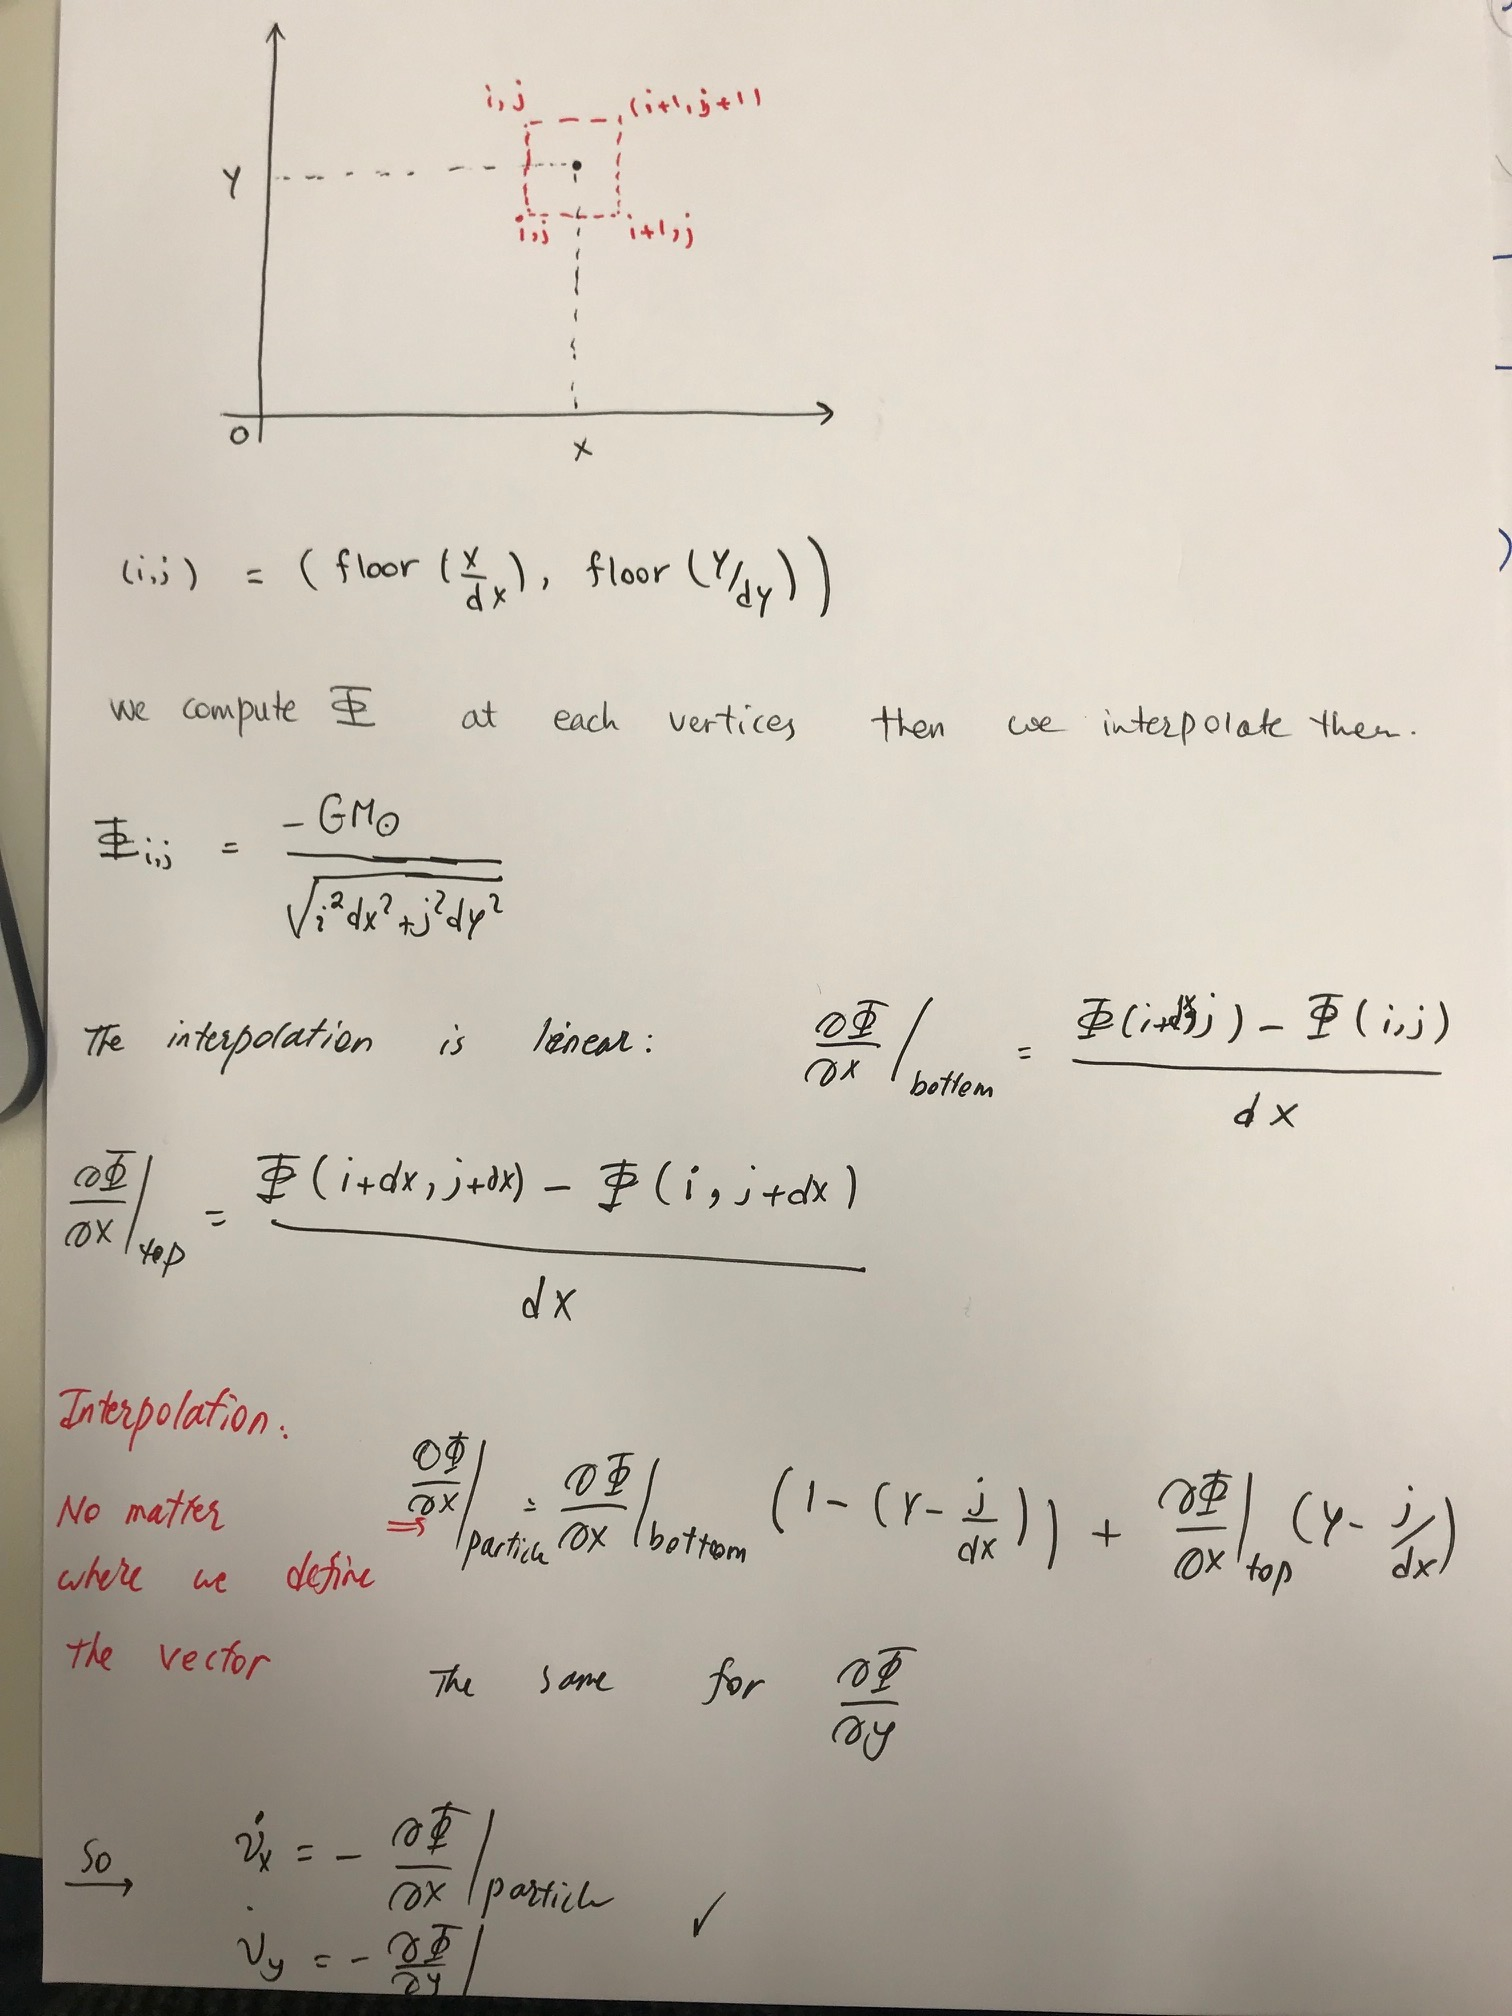
\includegraphics[scale=0.3]{./Images/Sch_correct.jpg} 
 \end{figure}
 \subsection{3 dimensional}
 The perihelion is computed by taking minimum $r= \sqrt{x^2+y^2}$ in the code.
The problem is illustrated in the figure. As it is clear, the problem is more complicated than before since the effect of each mass on the other is via the lattice vertices, so instead of one source we have basically 4 forces. We make some assumptions to simplify the problem, first we take one of the masses fixed by assuming $M  \gg m$, then we set the lattice coordinate by central mass $M$. Mass $m$ is allowed to freely move on the lattice and the lattice vertices have integer coordinates. Although in certain conditions the angular momentum of the system is conserved and we can define a plane, but we take general configuration first and then we restrict ourselves to some certain configurations.
       \begin{figure}[H]
 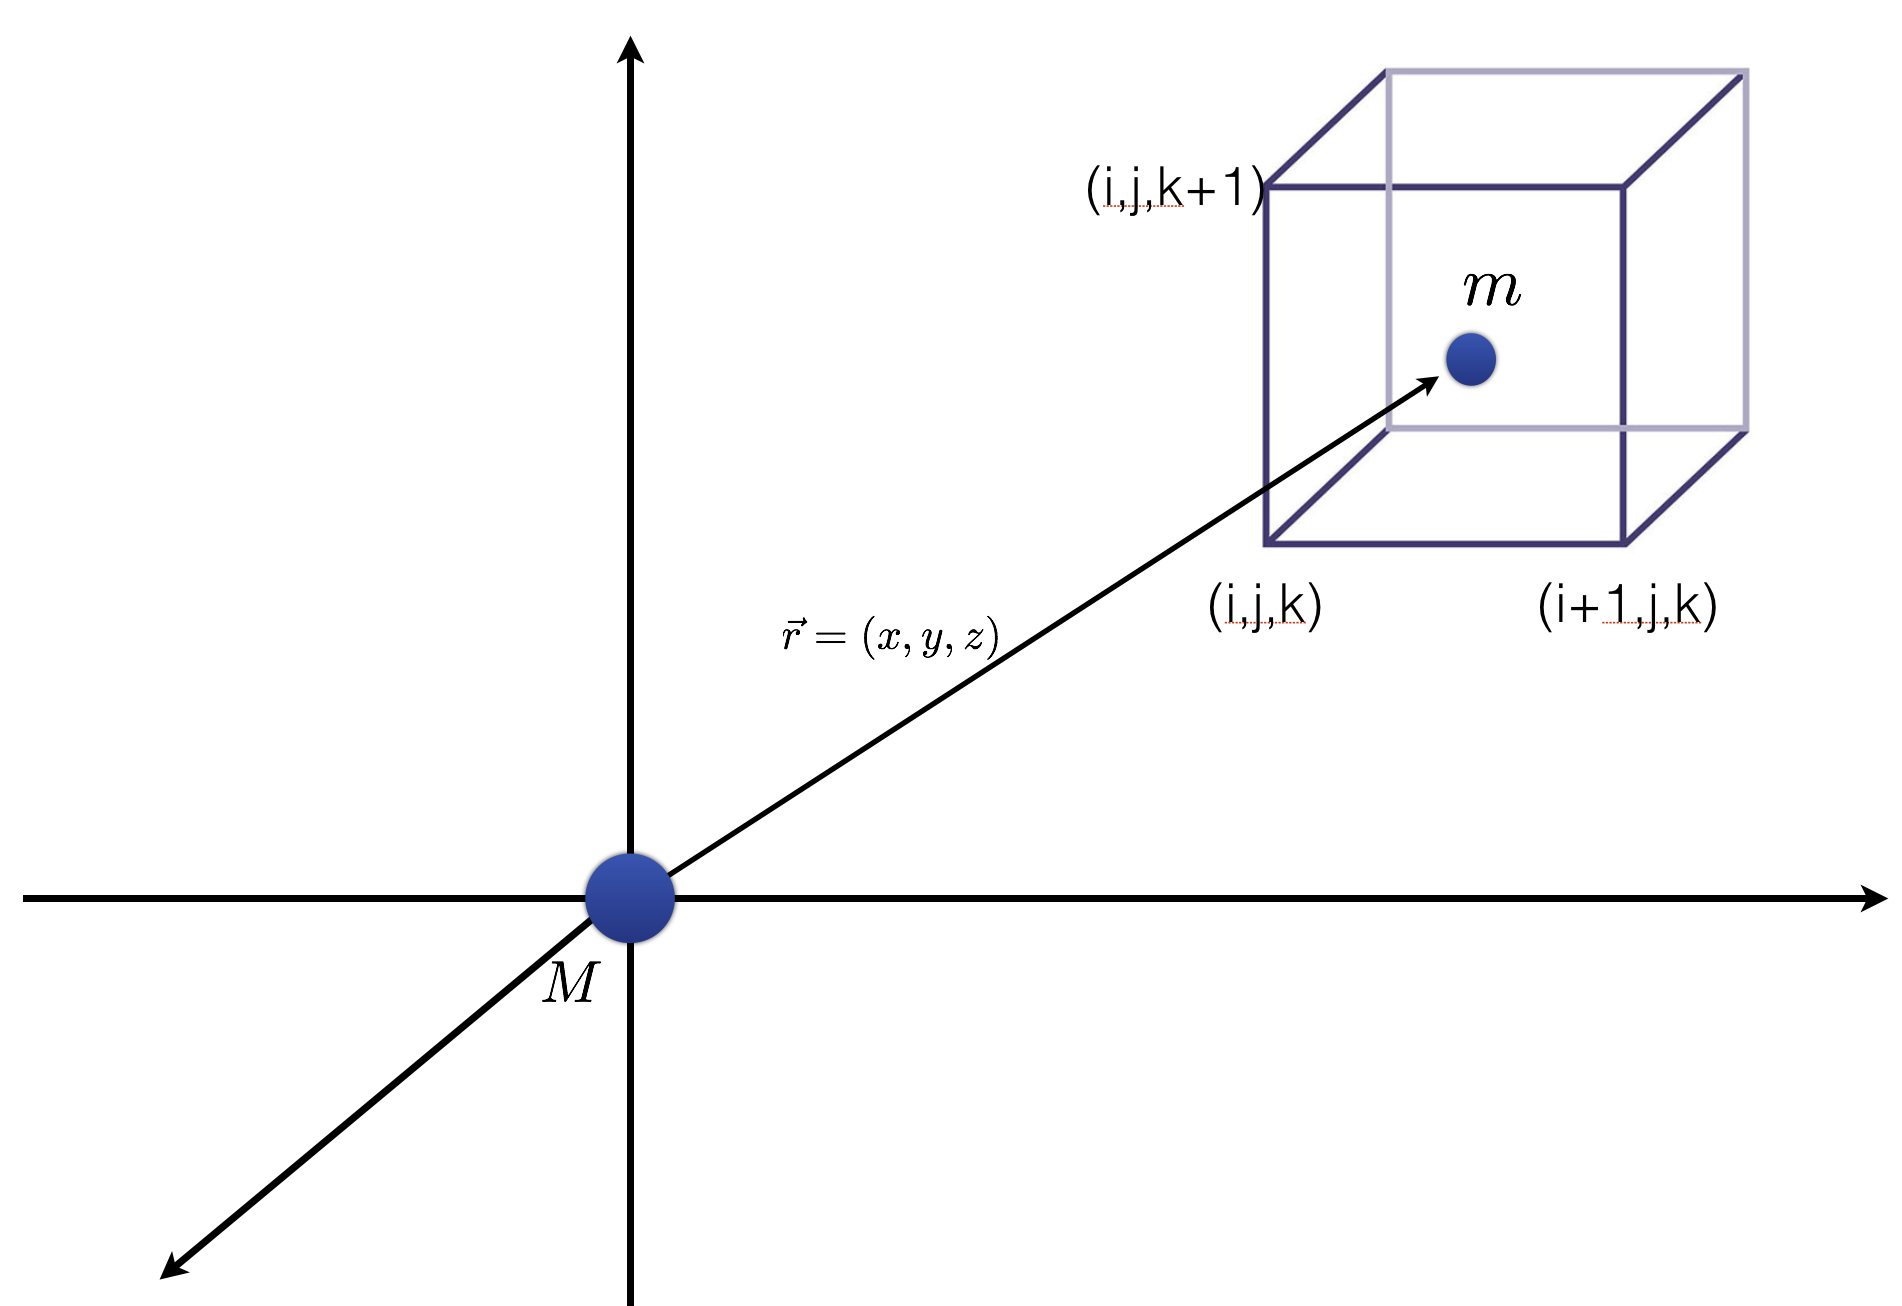
\includegraphics[scale=0.5]{./Images/Lattice_3d} 
 \end{figure}
 \subsection{Results}
Having the central object in the center and the other mass $m$ at position $(x,y,z)$, first we find the lattice which mass $m$ belongs to then the potential of $M$ on the cube vertices around the mass $m$  reads,
 \begin{align}
 &\Phi_{i,j,k} = -\frac{G M}{i^2	 + j^2 + k^2}
 \end{align}
 where $(i,j,k)$ is the position of one cube vertex and is obtained by taking the floor function of mass $m$ coordinate. The potentials are fixed so we only need to interpolate them on the planet position. 
 The way we do the interpolation is linear, meaning that the potential in the position of $m$ is,
 \begin{align}
& \Phi_{m}(x,y,z) =\sum_{ (i,j,k) \, \in \, \text{8 corners}  } \frac{\Phi_{i,j,k}}{2}  \Big[ \sqrt{1- (x-i)^2} +   \sqrt{1- (y-j)^2}  +  \sqrt{1- (z-k)^2} \Big ]
 \end{align}
Before writing the expression for the velocities and position updating, we would like to mention that angular momentum vector is not conserved necessarily, 
{\color{red} probably we can find some situations which the magnitude  of angular momentum vector is conserved and it just rotates?! or according to some symmetries we may be able to find a conserved quantity?! does the discretisation respect the symmetries? like conserving energy? probably it highly depends on the numerical method which update quantities in time!}   \\
The acceleration on  mass $m$ is obtained by taking the gradient of the potential,
\be
\dot{\vec v} = - \hat{e}_x \vec \nabla_x \Phi_{m} (x,y,z) -\hat{e}_y \vec \nabla_y \Phi_{m} (x,y,z) -\hat{e}_z  \vec\nabla_z \Phi_{m} (x,y,z)
\ee
Since  the lattice vertices are fixed we need to just take the gradient of weighting parts,
 \begin{align}
\dot{ \vec v} = \sum_{ (i,j,k) \, \in \, \text{8 corners}  } \frac{ \Phi_{i,j,k} }{2}  \;  \Big( \frac{x-i}{\sqrt{1-(x-i)^2} }, \; \frac{y-j}{\sqrt{1-(y-j)^2} },   \; \frac{z-k}{\sqrt{1-(z-k)^2} }   \Big)
 \end{align}
 Moreover,
 \be
 \vec v = \big( \dot x , \dot y, \dot z \big)
 \ee
Now lets start from some simple configurations, and try to obtain the results. For simplicity we consider a symmetric initial condition which  the source $M$ and mass $m$ are both at the $z=0$ plane and based on symmetry of the problem we have no motion in z direction, setting the initial conditions as mercury like object around the sun. \\
In the code we first find the lattice which the particle belongs to and then we compute the potential on the lattice vertices and interpolate on the mass position.

\section{General relativity}
The metric in a FLRW universe in Poisson gauge is,
\be 
ds^2=g_{\mu \nu} dx^{\mu}dx^{\nu}=[-c^2(1+2\Psi)d\tau ^2 -2B_i dx^i d \tau  + (1-2\Phi)\delta_{ij} dx^i dx^j +h_{ij}dx^i dx^j],
\ee

We can parameterize the scalar quantities in metric and write them as $e^{-2 \Phi'}$ and $e^{+2 \Psi'}$;
\be
ds'^2=g'_{\mu \nu} dx'^{\mu}dx'^{\nu}=[-c^2 e^{+2 \Psi'} d\tau'^2 -2B'_i dx'^i d \tau'  + e^{-2 \Phi'}\delta_{ij} dx'^i dx'^j +h'_{ij}dx'^i dx'^j],
\ee
The metric and Einstein equations in both parametrization are the same at linear order of perturbation and we have, \\
\be
\Psi'(\vec{x'},\tau')=\Psi(\vec{x},\tau),  \, \, \,
\Phi'(\vec{x'},\tau')=\Phi(\vec{x},\tau),  \, \, \,
ds'^2=ds ,  \, \, \,
x'^{\mu}=x^{\mu}
\ee
For the scalar degrees of freedom which is the case in Schwarzschild metric we can write;
\be 
ds^2=[-(1+2\Psi)c^2 d\tau ^2  + (1-2\Phi)\delta_{ij} dx^i dx^j], \label{metr1}
\ee
In new parameterization we have;
\be 
ds'^2=[-e^{+2\Psi'} c^2d\tau'^2  + e^{-2\Phi'} \delta_{ij} dx'^i dx'^j], \label{metr2}
\ee
If we expand the coefficients in weak field approximation we obtain equation [\ref{metr1}].
Here we try to obtain Einstein equations and Geodesic equation for new parameterization.\\
From now on we drop the prime " $'$ " from the new parameterization's coordinates but we should notice that the coordinate and the metric are different in the two parameterization. \\
%We calculate one equation by hand and the other by Mathematica,\\
%{\Large$:::::::::::::::::::::::::::::::::::::::::::::::::::::::::::::::::::::$}
\subsection{Einstein's equations}
In the background level the Einstein equations for both metric are similar.
\subsection{The geodesic equations, First order} 
To obtain first order geodesic equations we start from the classical action of massive test particle,
\be
\mathcal{A}=-m_o  \int \sqrt{-g_{\mu \nu} \dfrac{dx^{\mu}}{d \tau} \dfrac{dx^{\nu}}{d \tau} } d \tau=\int \mathcal{L} d \tau
\ee
Where $m_o$ is the mass of the object. If we use the metric definition  [\ref{metr1}] we can write;
\begin{align}
 \nonumber \mathcal{L}
=-m_oc \sqrt{1-(v/c)^2}\left(1+\dfrac{2 \Psi+2 (v/c)^2 \Phi} {1-(v/c)^2} \right)^{1/2}
\end{align}
The particle Lagrangian at linear order in perturbative potentials is,
\be
\mathcal{L}=-m_o c\sqrt{1-(v/c)^2} \left (  1+\dfrac{\Psi+(v/c)^2 \Phi}{1-(v/c)^2} \right)  +\mathcal{O}(\Phi^{2},\Psi^{2})
\ee
Where $v^2=v_i v^i$, $v_i=\delta_{ij}v^j$ and $v_i=\dfrac{dx_i}{d \tau}$ is the three velocity of particle.\\
The canonical conjugate momentum $q_i$ defined as $q_i=\dfrac{\partial \mathcal{L}}{\partial v^i}$;
\be
q_i=\dfrac{m_o}{\sqrt{1-(v/c)^2}} \left[  v_i \left( 1-2\Phi- \dfrac{\Psi+(v/c)^2 \Phi}{1-(v/c)^2} \right) \right]  +\mathcal{O}(\Phi^{2},\Psi^{2})\label{qi}
\ee
Just note that at the first order perturbation, for small enough $v$ we have $q_i=m v_i$. \\
We can rephrase the expression and get an equation for $v_i$,
%%%%%
\begin{align}
v_i=\dfrac{dx_i}{d \tau}=\dfrac{q_i}{\sqrt{q^2+m_o^2}} \left[1+\Psi +2\Phi+  \dfrac{-q^2}{q^2+m_o^2} \Phi  \right]+\mathcal{O}(\Phi^{2},\Psi^{2})   \label{v11}
\end{align}
%If we expand for small metric perturbations
%\begin{align}
%&\left( 1-v^2 \right) \left( v^2(-1+2 \Phi + \dfrac{\Psi+v^2 \Phi}{1-v^2}) \right) =\dfrac{m_o^2}{q^2}
%\end{align}
% Then using eq[\ref{q2}] and eq[\ref{qi}] we have,
 So we found an ODE to find the object's path.
 To find $q_i$ in the path equation we use the Euler-Lagrange equations $\dfrac{dq_i}{d \tau}=\dfrac{\partial \mathcal{L}}{\partial x^i}$.
 \begin{align}
 \dfrac{dq_i}{d \tau}=-\sqrt{q^2+m_o^2}  \left( \Psi_{,i}+\dfrac{q^2}{q^2+m_o^2c^2}\Phi_{,i}  \right)+\mathcal{O}(\Phi^{2},\Psi^{2})  \nonumber \\ &\label{part_Lx} 
 \end{align}
 Where $\Phi_{,i}=\partial \Phi/\partial x^i$. Using equations [\ref{v11}] and [\ref{part_Lx}] and applying Runge-Kutta algorithm, we can obtain $(x,y)$ position of particle in  time. We should notice that the geodesic equations are only valid to first order metric perturbations, but in principle we can define different parameterization of the metric and take the particle motion according to approximated geodesic equation. The exact derivation of equations is in appendix \ref{First order}. \\
 In the next subsection we obtain different linearized metric perturbation for Schwarzschild metric.
\subsection{ Schwarzschild metric}
Schwarzschild metric in isotropic coordinate is , 
%({\color{RedViolet}{why? Is this a good coordinate for comparing with numerical results?}})
\be 
ds^2=- \left ( \dfrac{1-\dfrac{r_S}{4r}}{1+\dfrac{r_S}{4r}} \right )^2 d\tau ^2  +(1+\dfrac{r_S}{4r})^4  \, \,[dr^2+r^2d \Omega ^2] ,
\ee
    If we compare the metric with equations [\ref{metr1}], [\ref{metr2}] we can derive the potentials for Schwarzschild case;
\be
\Psi_{exact}=-\dfrac{1}{2}+\dfrac{1}{2}\left ( \dfrac{1-\dfrac{r_S}{4r}}{1+\dfrac{r_S}{4r}} \right )^2
\ee
\be
\Phi_{exact}=\dfrac{1}{2}-\dfrac{1}{2} (1+\dfrac{r_S}{4r}  )^4
\ee
where $\Phi_{exact}$ and $\Psi_{exact}$ are the exact potentials. \\
In the weak field approximation we have $\Phi, \Psi \ll 1$  which is equivalent to $r\gg r_S$, so we can expand the expressions in terms of $\dfrac{r_S}{4r}$;
%\begin{align}
%%%%$
%\Psi_{approx}&=-\dfrac{1}{2}+\dfrac{1}{2} \dfrac{(1-\dfrac{r_S}{4r})^2}{(1+\dfrac{r_S}{4r})^2} = -\dfrac{1}{2}+\dfrac{1}{2} \left [ \dfrac{   1-2x+x^2   }{  1+2x+x^2  } \right] \\ &\nonumber
%\simeq  -\dfrac{1}{2}+\dfrac{1}{2}  (
%  1-2x+x^2  ) \left(1-2 x+3 x^2-4 x^3+5 x^4+O\left(x^5\right)\right )
%  \\ &\nonumber
%\simeq  -\dfrac{1}{2}+\dfrac{1}{2}  (
% 1-4 x+8 x^2-12 x^3+16 x^4+O\left(x^5\right) )
%   \\ &\nonumber
%\simeq    -2 x+4 x^2-6 x^3+8 x^4+O\left(x^5\right)
%\end{align}
%\begin{align}
%%$
%\Phi_{approx}&=\dfrac{1}{2}-\dfrac{1}{2} (1+\dfrac{r_S}{4r}  )^4= \dfrac{1}{2}-\dfrac{1}{2} (1+x  )^4 \\ &\nonumber
%\simeq -2 x-3 x^2-2 x^3-\frac{x^4}{2}+O\left(x^5\right)
%\end{align}
%So the related $\Phi$ and $\Psi$ for Schwarzschild metric are;
\be
\Psi_{approx} \simeq -2 \dfrac{r_S}{4r} +4 (\dfrac{r_S}{4r})^2-6 (\dfrac{r_S}{4r})^3+8 (\dfrac{r_S}{4r})^4+O\left((\dfrac{r_S}{4r})^5\right)
\ee
\be
\Phi_{approx} \simeq  -2 \dfrac{r_S}{4r}-3 (\dfrac{r_S}{4r})^2-2 (\dfrac{r_S}{4r})^3-\frac{1}{2}(\dfrac{r_S}{4r})^4+O\left((\dfrac{r_S}{4r})^5\right)
\ee
\\
For the other parameterization of the perturbed metric, equation [\ref{metr2}], we have;
\be
e^{+2 \Psi'}=\left ( \dfrac{1-\dfrac{r_S}{4r}}{1+\dfrac{r_S}{4r}} \right )^2
\ee
\be
e^{-2 \Phi'}=(1+\dfrac{r_S}{4r})^4
\ee
If we expand the expressions for $\Phi', \Psi'\ll 1$  or equivalently $r\gg r_S$ ;
%\begin{align}
%%$
%&+2 \Psi'= \ln{ \left ( \dfrac{1-x}{1+x} \right )^2}\rightarrow \Psi'= + \ln{ \left ( \dfrac{1-x}{1+x} \right )}
%\\ \nonumber & \Longrightarrow  \Psi' \simeq -2 x-\frac{2 x^3}{3}-\frac{2 x^5}{5}+O\left(x^6\right)
%\end{align}
%\begin{align}
%%$
%&-2 \Phi'=\ln{(1+x)^4} \rightarrow \Phi'=-2\ln{(1+x)}
%\nonumber \\ &
% \Longrightarrow \Phi' \simeq -2 x+x^2-\frac{2 x^3}{3}+\frac{x^4}{2}-\frac{2 x^5}{5}+O\left(x^6\right)
%\end{align}
%The related $\Phi'$ and $\Psi'$ in the exponential parameterization are;
\be 
\Psi_{param} \simeq -2 \dfrac{r_S}{4r}-\frac{2 }{3}(\dfrac{r_S}{4r})^3-\frac{2 }{5}(\dfrac{r_S}{4r})^5+O\left((\dfrac{r_S}{4r})^6\right)
\ee
\be 
\Phi_{param} \simeq -2 \dfrac{r_S}{4r}+(\dfrac{r_S}{4r})^2-\frac{2 }{3} (\dfrac{r_S}{4r})^3+\frac{1}{2} (\dfrac{r_S}{4r})^4-\frac{2 }{5}(\dfrac{r_S}{4r})^5+O\left((\dfrac{r_S}{4r})^6\right)
\ee
Using different potentials in approximated geodesic equation we can check the accuracy of each by comparing with general relativity solution.
\subsection{Geodesic equations-Beyond first order approximation}
The exact, non linear self contained geodesic equations based on the exact calculation same as before are,\\
\be
\dfrac{dq_i}{d \tau}= -m_o \sqrt{1-v^2}  \left(      \frac{ v^2 \Phi _{,i}+ \Psi_{,i}}{ 1-v^2 }  \right) \left(1+\frac{2 v^2 \Phi +2 \Psi }{1-v^2} \right)^{-1/2}  \label{q_iful_1}
\ee
\begin{align}
\dfrac{d x_i }{d \tau}=\dfrac{q_i \sqrt{1-v^2/c^2}}{m_o } \; \dfrac{\sqrt{1+\dfrac{2 \Psi+2( v^2/c^2) \Phi}{1-v^2/c^2}  }  }  {1-2 \Phi}  \label{v_iful_1}
 \end{align}
%The presence of $v^2$ in the right hand side of the equation [\ref{v_iful_1}] cause the error in the solustions which cannot be easily estimated according to non linear nature of the equations.
First we obtain a non linear algebraic equation for $v^2$ from  [\ref{v_iful_1}],
\begin{align}
&q_iq^{i}=\dfrac{m_o^2 v_iv^i }{1-v^2/c^2}   \;   \dfrac{(1-2 \Phi)^2}{(1+\dfrac{2 \Psi+2 (v^2/c^2) \Phi}{1-v^2/c^2})}  \nonumber \\ &
v^2=\left (\frac{1}{c^2}+\dfrac{m_o^2(1-2 \Phi)^2}   {q^2(1+\dfrac{2 \Psi+2(v^2/c^2)\Phi}{1-v^2/c^2})}  \right)^{-1} \label{v2ex_1}
\end{align}
We should be very careful to do the expansion consistently, because in $v^2$ there are $v^2$ and $q^2$ terms which can be any order in terms of potentials. So we should expand all the terms to second order and then simplify the equations. We start from $v^2$ and then substitute itself into $v^2$ and repeat the procedure to have an expression for $v^2$ in terms of $q^2$ and without $v^2$ terms. The complete calculations can be found in appendix \ref{geodesic_beyond}.
\begin{align}
v^2= \frac{q^2 c^2}{q^2+m_o^2 c^2} \text{\Huge [}1
&+
\frac{2    \left(2 m_o^2 c^2 \Phi +m_o^2 c^2 \Psi +q^2 \Phi +q^2 \Psi \right)}{m_o^2 c^2+q^2}
+
\nonumber \\ &+
\frac{4   \left(3 m_o^4 c^4 \Phi ^2+2 m_o^4  c^4 \Phi  \Psi +3 m_o^2 c^2 q^2 \Phi ^2+3 m_o^2 c^2 q^2 \Phi  \Psi +q^4 \Phi ^2+q^4 \Phi  \Psi \right)}{\left(m_o^2 c^2+q^2\right)^2} \text{\Huge ]}
%+ \mathcal{O}(\Phi^{3},\Psi^{3}) 
\end{align}
By substituting $v^2$ in the equations [\ref{q_iful_1}] and  [\ref{v_iful_1}] we have second order geodesic equations. Note that it is not necessary to expand the ODEs after $v^2$ substitution, because anyway the order of equations do not change and is second order. So we have two ways to get second order geodesic equations results. \\
The first set of equations are;
\begin{align}
v^2= \frac{q^2 c^2}{q^2+m_o^2 c^2} \text{\Huge [}1
&+
\frac{2    \left(2 m_o^2 c^2 \Phi +m_o^2 c^2 \Psi +q^2 \Phi +q^2 \Psi \right)}{m_o^2 c^2+q^2}
+
\nonumber \\ &+
\frac{4   \left(3 m_o^4 c^4 \Phi ^2+2 m_o^4  c^4 \Phi  \Psi +3 m_o^2 c^2 q^2 \Phi ^2+3 m_o^2 c^2 q^2 \Phi  \Psi +q^4 \Phi ^2+q^4 \Phi  \Psi \right)}{\left(m_o^2 c^2+q^2\right)^2} \text{\Huge ]}\label{v2_1}
%+ \mathcal{O}(\Phi^{3},\Psi^{3}) 
\end{align}
\be
\dfrac{dq_i}{d \tau}= -m_o \sqrt{1-v^2}  \left(      \frac{ v^2 \Phi _{,i}+ \Psi_{,i}}{ 1-v^2 }  \right) \left(1+\frac{2 v^2 \Phi +2 \Psi }{1-v^2} \right)^{-1/2}  \label{setI1}
\ee
\begin{align}
\dfrac{d x_i }{d \tau}=\dfrac{q_i \sqrt{1-v^2/c^2}}{m_o } \; \dfrac{\sqrt{1+\dfrac{2 \Psi+2( v^2/c^2) \Phi}{1-v^2/c^2}  }  }  {1-2 \Phi}   \label{setI2}
 \end{align}
On the other hand by substituting $v^2$ into the geodesic equations and expanding to second order in potentials we obtain the below equations for the object's orbit.

 \begin{align}  \label{setII2}
&\dfrac{dq_i}{d \tau}= -c \sqrt{m_o^2 c ^2+q^2} \left(\Psi_{,i} +\Phi_{,i} \dfrac{q^2}{m_o^2 c^2+q^2}\right)+
 \\ \nonumber &
 +c\left [ \frac{m_o^4 c^4 \Psi   \Psi_{,i}-4 m_o^2 c^2 q^2 \Phi  \Phi_{,i}-m_o^2 c^2 q^2 \Phi  \Psi_{,i}-m_o^2 c^2 q^2 \Phi_{,i} \Psi +2 m_o^2  c^2 q^2 \Psi  \Psi_{,i} -3 q^4 \Phi  \Phi_{,i}-q^4 \Phi  \Psi_{,i}-q^4 \Phi_{,i} \Psi +q^4 \Psi  \Psi_{,i}}{\left(m_o^2+q^2\right)^{3/2}} \right ]+\mathcal{O}(\Phi^3..)  \label{setII1}
\end{align}
 \begin{align}
v_i=& \dfrac{q_i c}{\sqrt{q^2+m_o^2 c^2}} \left[1+\Psi +2\Phi+  \dfrac{-q^2}{q^2+m_o^2 c^2} \Phi  \right]+ \nonumber \\ &
\frac{q_i  c  \left(8 m_o^4 c^4 \Phi ^2+4 m_o^4 c^4 \Phi  \Psi -m_o^4 c^4 \Psi ^2+8 m_o^2 c^2 q^2 \Phi ^2+6 m_o^2 c^2 q^2 \Phi  \Psi -2 m_o^2 c^2 q^2 \Psi^2 +3 q^4 \Phi ^2+2 q^4 \Phi  \Psi -q^4 \Psi ^2\right)}{2 \left(m_o^2 c^2+q^2\right)^{5/2}} +\mathcal{O}(\Phi^3,\Psi^3,..)
 \end{align}
%So we use equation [\ref{v2ex}] to have $v^2_{n+1}$ from $v^2_n$ and the potentials in $n$th step of Runge-Kutta algorithm, then we estimate $v_i$ according to equations [\ref{v_iful}] and [\ref{q_iful}].

\section{First order geodesic equations and different potentials results}
%Here we try to compare the accuracy of different potentials within approximated geodesic equation.\\
%The approximated GR equations of motion  where we neglect the second order terms of potentials are written as below;
%\begin{align}
%&\dfrac{d\vec{r}}{dt}=\dfrac{\vec{q}}{\sqrt{q^2+m_o^2}} \left[ 1+\Psi+ \left( 2-\dfrac{q^2}{q^2+m_o^2} \right) \Phi \right]
%\end{align}
%\begin{align}
%&\dfrac{d\vec{r}}{dt}=\dfrac{\vec{q}}{\sqrt{q^2+m_o^2}} \left[ 1+\Psi+ \left( 2-\dfrac{q^2}{q^2+m_o^2} \right) \Phi \right]
%\end{align}
%\begin{center} [htbp!]
%    \begin{tabular}{ |p{9cm}||p{1.5cm}|p{4cm}|p{4cm}| }
%    \hline
%   Model  & Run time (sec) & working precision  &  Perihelion advance (Arcsecond/Century)    \\ \hline
%    % & Summary
%   The exact Differential equation & 2 &40&42.96 \\
%      The approximated Geodesic-Exact potentials   &245.13&90&420.54  \\
%    Approximated standard potentials    & 271.47 &90&420.54  \\
%     Approximated new potentials     & 294.19 &90&435.47  \\

%  \hline
%    \end{tabular}
%\end{center}
%\be
%\text{$\Psi $1app}(\text{r$\_$})\text{:=}-6 \left(\frac{\text{Rsch}}{4 r}\right)^3+4 \left(\frac{\text{Rsch}}{4 r}\right)^2-\frac{2 \text{Rsch}}{4 r}
%\ee
Here we check the accuracy of different potentials in  approximated geodesic equation via comparing with the exact GR solution for Schwarzschild metric equations of motion.
One interesting test is measuring the perihelion advance in each case and comparing with the GR perihelion advance which is obtained,
\be
\delta \theta \approx \dfrac{6 \pi G ^2 M^2}{c^2 l^2}
\ee
Where $\delta \theta$ is perihelion advance per orbit, $l$ is angular momentum per object's mass and $M$ is central object's mass.\\
To go in different regime we define a parameter $\alpha$ which scales the physical quantities as following,
\begin{align}
&M \rightarrow \alpha M \\
 &v_{per} \rightarrow \sqrt{\alpha} v_{per}  \\
 &T \rightarrow \dfrac{T}{\sqrt{\alpha}}
\end{align}
$T$ is the object's period, $v_{per} $ is the perihelion speed of the object and $M$ is the central object's mass. By $\alpha$ we can go to the strong/weak limit  while keeping one period orbit in time $\dfrac{T}{\sqrt{\alpha}}$ .
\\
The initial conditions for the problem are,
\begin{align}
&x_0=R \\
&y_0=0 \\
&q_x=R  \,v_{per}\\
&q_y=0
\end{align}
To compare the results with Mercury observations we use Mercury's facts %\ref{facts}
\begin{align}
&M_{mercury}=3.285 \times 10^{24}  \text{  kg}\\
&T=87.96 \text{  days}\\
&v_{per}=58.98 \text{  $k m/s$}\\
&R=46 \times 10^9   \text{  $ m$}\\\
&M_{sun}=1.99 \times 10^{30}  \text{  $ kg$}\\\
\end{align}
Then we try to plot different figure to compare different potentials. In figure \ref{GRperpos} we plot the first and 415th orbit of Mercury like object with coefficient $ \alpha=10^{-2}$ which goes under exact Schwarzschild potentials. it can be seen that we cannot distinguish between two orbits with eye. We choose 415th orbit because in $\alpha=1$ it is equivalent for 1 century. \\

%\begin{center} 
%    \label{facts}
%    \captionof{table}{Mercury facts }
%    \begin{tabular}{ |p{9cm}||p{1.5cm} }
%    \hline
%
%  \hline
%    \end{tabular}
%\end{center}
\end{document}

